% Observational Production Functions for Language Models and the Measurement of Algorithmic Progress.
% Companion paper to "What Optimizing Labs Reveal: Scaling Laws as Production Functions" (paper/main.tex).
% Round-3 writer (companion), 2026-09-24. Built from paper/sections/appendix_observational.tex (v2 Online Appendix E),
% the ra4_obsfix, m4_observational, m5_progress and m6_montecarlo memos and reviews, and the proofs of v2 Appendix A.
% Numbers and sources: paper/notes/writer3_companion.md. Compile here with ../../tools/tectonic -X compile observational.tex
\documentclass[AER,finalmode]{AEA}
\usepackage{natbib}
\let\proof\relax\let\endproof\relax
\usepackage{amsmath,amssymb,amsthm}
\usepackage{graphicx}
\usepackage{booktabs}
\usepackage{dcolumn}
\usepackage{multirow}
\usepackage{array}
\usepackage{xcolor}
\usepackage[section]{placeins}% keep floats inside their section
\usepackage[colorlinks=true,citecolor=blue!50!black,linkcolor=blue!50!black,urlcolor=blue!50!black]{hyperref}
\hypersetup{pdftitle={Observational Production Functions for Language Models and the Measurement of Algorithmic Progress},pdfauthor={Yigit Okar}}
\graphicspath{{../../output/figures/}}
\newtheorem{proposition}{Proposition}
\newtheorem{lemma}{Lemma}
\newtheorem{corollary}{Corollary}
\theoremstyle{definition}
\newtheorem{definition}{Definition}
\theoremstyle{remark}
\newtheorem{remark}{Remark}
\draftSpacing{1.5}
\providecommand{\E}{\mathbb{E}}
\providecommand{\Var}{\operatorname{Var}}
\providecommand{\Cov}{\operatorname{Cov}}

% Working-paper running heads (as in the main paper): author, short title and page, not the journal's heads.
\makeatletter
\issueName{Working Paper}
\def\ps@headings{%
  \leftskip=0pt\rightskip=0pt
  \let\@oddfoot\@empty
  \let\@evenfoot\@empty
  \def\@oddhead{{\small\textit{\MakeUppercase{Okar\hfil\@shortTitle\hfil\thepage}}}}%
  \def\@evenhead{{\small\textit{\MakeUppercase{\thepage\hfil\@issueName\hfil\@pubMonth\ \@pubYear}}}}}
\pagestyle{headings}
% Table numbers end with a period, like figure numbers, instead of the class default dash (author's style rule).
\def\fnum@table{\tablename\nobreakspace\thetable.\nobreakspace}
\makeatother

\begin{document}

\title{Observational Production Functions for Language Models and the Measurement of Algorithmic Progress}
\shortTitle{Observational Production Functions}
\author{Yigit Okar\thanks{Care AI (email: okar.yigit@gmail.com). This paper is a companion to \citet{okar2026what},
which estimates the technology of training language models from designed experiments; its material appeared as a
section of an earlier version of that paper. This paper was produced in close collaboration with Claude, an AI system
developed by Anthropic. Claude designed and carried out the analysis (the data construction, the theory and its
verification, the estimation, the simulations and the replication of \citet{ho2024algorithmic}) and drafted the paper
with the author, who takes responsibility for its content. The author posed the research question and made the
project's decisions on scope, disclosure and publication. The author gratefully acknowledges this contribution; under
the AEA's authorship policy an AI system cannot be listed as an author. The author thanks the authors of
\citet{ho2024algorithmic} for making their data and code public, which made the exact replication in
Section~\ref{sec:progress} possible, and will share the findings of that section with them before circulating this
paper and report their response in a revised version. Data and code availability: all data used in the paper are
publicly available. The replication package (github.com/yigitokar/scaling-laws-as-production-functions, release
\texttt{v4}) reproduces the tables and figures from the raw downloads with fixed random seeds. For sources that carry
no license permitting redistribution (Epoch AI's digitization of the Chinchilla runs and the Farseer run files), it
provides download scripts and SHA-256 checksums of the files we used in place of
the data.}}
\date{September 2026}
\pubMonth{September}
\pubYear{2026}

\begin{abstract}
Estimates of returns to compute and algorithmic progress in language models come mostly from models that developers
chose to train. We ask what such data identify. Matched to the design of released models, cross-lab returns to compute
do not differ detectably from an experimental benchmark in a low-power test; the split between parameters and data is
not reliably estimated. In the leading data on algorithmic progress, the rate is weakly identified: bias and rate of
technical change trade off along a ridge. Rebalancing away from under-training raised the training-cost efficiency of
large models 1.1 to 4.9-fold, depending on the technology.
\end{abstract}
\JEL{C51, D24, L86, O33, O47}
\Keywords{production functions, transmission bias, algorithmic progress, productivity dispersion, biased technical
change, large language models}

\maketitle

% =====================================================================================================================
Much of what economists and forecasters know about how language models improve with scale, and about how fast the
methods for training them improve, comes from models that their developers chose to train. Throughout, we call the
firms and research groups that train language models ``labs''; the term covers both the developers that release models
and the designers of the training experiments that measure the technology. Observational scaling studies regress the
benchmark scores of models released by many labs on their parameters and training tokens
\citep{ruan2024observational,maiapolo2024sloth,owen2024predictable,mertens2026secret}. The leading estimate of
algorithmic progress regresses the perplexity of published models on their inputs and publication dates
\citep{ho2024algorithmic}. To an economist these are production-function regressions on observational data. The labs
chose their inputs knowing something about their own productivity. That is the setting in which
\citet{marschak1944random} showed least squares to be biased \citep[see][]{griliches1998production}, and
\citet{whitfill2025note} and \citet{konig2026validity} warn that the estimates for language models may be
confounded.

This paper asks what such data can identify. The industry offers a check that economists who study production rarely
have. Besides observational data there are designed experiments: public sweeps in which researchers train models over
grids of parameters and tokens with a fixed recipe
\citep{hoffmann2022training,bhagia2024establishing,gadre2024language}. A companion paper \citep{okar2026what} uses such
experiments to estimate the training technology and reads labs' choices through it. Here we use them as a benchmark
for observational estimators, and we derive what cross-lab data can and cannot deliver when labs choose inputs knowing
their productivity.

We have five findings. First, returns to compute survive a comparison with the experiments once the design is matched.
The technology is strongly curved, and released models sit where an extra training token is worth little, so a
comparison of observational estimates with global experimental elasticities mistakes curvature for bias. We therefore
evaluate the experimental technology at the inputs of the released models and apply each estimator to both sets of
outputs. On 57 models the compute elasticity of HellaSwag performance differs by $-0.001$, with a standard error of
0.041. This is a failure to reject in a joint test of low power, not evidence of unbiasedness: the bias detectable with
80 percent power is 37 percent of the benchmark. The split of returns between parameters and data is not reliably
estimated.

Second, compute is measured well enough that errors in variables do not matter, but the standard remedies for
transmission bias cannot be applied. The available instruments are weak or fail their exclusion restrictions, and
product lines are too short for dynamic-panel estimators. Proxy inversion fails for structural reasons that we
establish: at given compute, Hicks-neutral productivity does not move the input mix, and compute cannot proxy
productivity because the inputs on the expansion path are functions of compute alone.

Third, productivity dispersion across model families is about as large as within US manufacturing industries when it
is measured in output units. Measured in compute-equivalent units, the 90--10 ratio is 7 to 24, against 1.9 in
manufacturing. Because returns to compute are small, the two unit systems differ by a large factor, and comparisons with
other industries are a choice of cardinalization rather than a finding.

Fourth, in the data of \citet{ho2024algorithmic} the rate of algorithmic progress is weakly identified. The sample is
off the expansion path, and the estimates lie on a ridge along which the bias of technical change trades off against
its rate, the identification problem of \citet{diamond1978measurement}. The profile-likelihood interval for the doubling
time of effective compute runs from 4.1 to 40.5 months, and a restriction on the bias buys most of the precision:
imposing Hicks neutrality gives 9 to 12 months. We reproduce the published estimates exactly from the authors' data and
code. On this ridge the reported point depends on the optimizer's stopping rule: run to convergence, the authors'
objective falls from 0.0518 to 0.0507 while the fit changes by 0.27 percent, and the doubling time moves from 8.7 to
6.1 months. The finding concerns numerical optimization on a flat objective, not the order of magnitude of progress.

Fifth, counting only the elimination of under-training, the move from the allocations implied by the scaling law of
\citet{kaplan2020scaling} to those of \citet{hoffmann2022training} raised the training-cost efficiency of large models
by a factor of 2.0 under the reference technology of the companion paper (1.1 to 4.9 across 14 technologies).
\citet{gundlach2025origin} define the compute-equivalent gain of such rebalancing and show that continuing the earlier
rule would cost about tenfold at 2025 frontier compute. Our counterfactual agrees; what we add is that the gain
realized between the two eras was a fraction of that counterfactual.

Section~\ref{sec:theory} collects the theory that organizes these findings. Transmission from productivity to compute
biases returns to compute with the sign of the compute response, upward when more productive labs raise more compute
and downward when labs train to a common capability target, but it leaves the allocation exponent unbiased. The
forward--reverse bracket familiar from errors in variables \citep{klepper1984consistent} fails under funding, and
selection on released outcomes attenuates transmission bias and can reverse it. If compute-optimal models were observed
at several dates, the drift in their ratio of tokens to parameters would identify the sign of the bias of technical
change, though not its size, because the elasticity of substitution between parameters and data is below one at
interior optima. Growth-accounting corollaries characterize when compute-equivalent gains are the same at every scale,
how regressions of frontier loss on compute without time effects attribute progress to scale \citep{nagy2013statistical},
and how an equal-weight productivity residual misattributes input shifts to productivity \citep{hall1988relation}.

These are classic questions of production economics. Estimators of production functions under endogenous inputs
\citep{olley1996dynamics,levinsohn2003estimating,ackerberg2015identification,gandhi2020identification} are usually
judged by their assumptions, because the truth is unknown. Here part of the truth is measured, so the exercise is a
validation of observational estimators against experimental benchmarks, in the tradition of
\citet{lalonde1986evaluating} and \citet{dehejia1999causal}, but across populations
\citep{hotz2005predicting,todd2006assessing}: the experimental recipes are not the released models' recipes. The
measurement of productivity dispersion \citep{syverson2004product,syverson2011determines} and of the bias of technical
change \citep{diamond1978measurement,leonledesma2010identifying} meet a technology whose returns to its composite input
are far from constant. For the literature on progress in machine learning
\citep{erdil2022algorithmic,sevilla2022compute,ho2024algorithmic,gundlach2025origin,whitfill2025note}, the paper
supplies the identification results and the benchmark. The general lesson reaches beyond language models. Wherever
producers choose inputs knowing their productivity and designed variation exists, as in agronomic field trials or
sweeps of chip designs, matching the observational design to the experimental one is what makes a validation
informative. Where designed variation does not exist, what observational data lack is variation transverse to the
expansion path, and no estimator supplies it.

The rest of the paper proceeds as follows. Section~\ref{sec:theory} sets out the theory, Section~\ref{sec:data} the
data. Section~\ref{sec:matched} compares observational and experimental returns to compute, Section~\ref{sec:compute}
discusses the measurement of compute and the standard remedies, and Section~\ref{sec:tfp} measures productivity
dispersion. Section~\ref{sec:progress} revisits the estimation of algorithmic progress, Section~\ref{sec:allocative}
separates allocative from technical change, and Section~\ref{sec:conclusion} concludes. The
appendices collect the proofs (Appendix~\ref{app:proofs}), details of the data (Appendix~\ref{app:data}), the
simulations (Appendix~\ref{app:mc}) and additional tables (Appendix~\ref{app:tables}).

% =====================================================================================================================
\section{What Cross-Lab Data Can Identify}\label{sec:theory}

\subsection{The Technology}\label{sec:tech}

We use the technology of \citet{hoffmann2022training} with productivity terms, in the generalized form of
\citet{okar2026what}. A training run uses $N$ parameters and $D$ training tokens (tokens processed, including
repetitions) and attains held-out cross-entropy
\begin{equation}\label{eq:tech}
L=E+e^{-\omega}\Big[A\big(e^{\psi_N}N\big)^{-\alpha}+B\big(e^{\psi_D}D\big)^{-\beta}\Big]^{\kappa}e^{\zeta},
\qquad A,B,\alpha,\beta,\kappa>0,
\end{equation}
where $E$ is irreducible loss, $\omega$ is Hicks-neutral productivity, $\psi_N$ and $\psi_D$ are factor-augmenting
productivity, and $\zeta$ is noise. The Chinchilla form is $\kappa=1$. The lab knows $(\omega,\psi_N,\psi_D)$ when it
chooses inputs, but not $\zeta$. Lower-case letters denote logs: $n=\ln N$, $d=\ln D$ and $c=\ln C$, with training
compute $C=6ND$, so that $c=\ln6+n+d$; $M\equiv D/N$ is the number of tokens per parameter. The output index is
$y\equiv-\ln(L-E)=\omega+F(n+\psi_N,d+\psi_D)-\zeta$, with $F(n,d)\equiv-\kappa\ln(Ae^{-\alpha n}+Be^{-\beta d})$.

The output elasticities are $\varepsilon_N\equiv\partial y/\partial n$ and $\varepsilon_D\equiv\partial y/\partial d$,
and their ratio is the wedge $w\equiv\varepsilon_N/\varepsilon_D$. A run on the training-cost-minimizing expansion
path has $w=1$. Along that path parameters grow with compute at elasticity $a\equiv\beta/(\alpha+\beta)$, reducible
loss falls with compute at elasticity $\gamma\equiv\kappa\alpha\beta/(\alpha+\beta)$, which we call the frontier
elasticity, and the elasticity of substitution between parameters and data is $\sigma^*\equiv2/(2+\alpha+\beta)$.
Productivity enters the allocation through the bias index $\chi\equiv\beta\psi_D-\alpha\psi_N$ and output through
compute-equivalent productivity $\Omega\equiv\omega+\gamma(\psi_N+\psi_D)$.

\begin{lemma}[Allocation and allocative loss]\label{lem:alloc}
\begin{enumerate}
\item[(i)] At given compute, the inputs that maximize $y$ satisfy
$n^*=\ln G+a(c-\ln6)+\chi/(\alpha+\beta)$ and $d^*=c-\ln6-n^*$, where $G\equiv(\alpha A/\beta B)^{1/(\alpha+\beta)}$,
and attain $y^*=\Omega+\gamma(c-\ln6)-\ln K-\zeta$ for a constant $K$. Hicks-neutral productivity does not enter the
allocation.
\item[(ii)] For any run, $\ln w=\tfrac{\alpha+\beta}{2}\ln\big(M/M^*(C)\big)$, where $M^*(C)$ is the compute-optimal
ratio at the run's compute for the lab's own productivity.
\item[(iii)] Let $C_{\min}(R)$ be the least compute that attains the run's reducible loss $R=L-E$. Then
\begin{equation}\label{eq:ce}
\frac{C}{C_{\min}(R)}=\Big(\frac{\alpha+\beta w}{\alpha+\beta}\Big)^{(\alpha+\beta)/(\alpha\beta)}w^{-1/\alpha},
\end{equation}
which depends on neither $(A,B,E,\kappa)$ nor productivity. To second order,
$\ln(C/C_{\min})=(\ln w)^2/[2(\alpha+\beta)]$.
\end{enumerate}
\end{lemma}

Part (iii) makes allocative efficiency measurable: the compute a run spends beyond the cheapest way of reaching its own
loss is a function of its wedge alone. The loss is a Harberger triangle whose area is governed by the elasticity of
substitution, since $2(\alpha+\beta)=4(1-\sigma^*)/\sigma^*$.

Why would a wedge differ from one? \citet[Proposition 1]{okar2026what} shows that a lab that values compactness (because
it serves the model, because its users bear the serving cost and adoption responds to it, or because it targets a
deployment tier) chooses $w>1$, and that serving demand cannot produce $w<1$ as long as serving expenditure rises with
model size at given quality. Wedges below one arise from optimization against a different technology, for example the
law of \citet{kaplan2020scaling}, from a binding cap on training data, or from costs of data. For an econometrician who
ignores factor-augmenting productivity, the measured wedge is $we^{-\chi}$. Most open-weight models released since 2023
are trained beyond training-cost minimization \citep{okar2026what}, so released models are far from the expansion
path.

\subsection{Transmission and Selection}\label{sec:transmission}

Consider first runs on the expansion path of a common technology with Hicks-neutral productivity only. By
Lemma~\ref{lem:alloc}(i), $y_i=\omega_i+\gamma c_i-\zeta_i$ up to a constant. Compute responds to productivity through
$c_i=\pi_0+\pi_1\omega_i+\eta_i$, with $(\omega,\eta,\zeta)$ mutually uncorrelated and variances
$V_\omega,V_\eta,V_\zeta$. Three rules are special cases: exogenous budgets ($\pi_1=0$); funding, under which more
productive labs raise more compute ($\pi_1>0$); and a capability target, under which every lab trains until it reaches
a common loss ($\pi_1=-1/\gamma$).

\begin{proposition}[Transmission]\label{prop:transmission}
\begin{enumerate}
\item[(i)] The least-squares slope of $y$ on $c$ converges to $b_f=\gamma+\pi_1V_\omega/(\pi_1^2V_\omega+V_\eta)$; its
bias has the sign of $\pi_1$. Under a capability target, $b_f=\gamma V_\eta/(V_\omega/\gamma^2+V_\eta)\in[0,\gamma)$,
and if every lab hits the target exactly ($V_\eta=0$), cross-lab data carry no information about $\gamma$.
\item[(ii)] The residual variance is $V_\omega V_\eta/\Var(c)+V_\zeta$, so productivity dispersion measured from
residuals is understated whenever $\pi_1\neq0$.
\item[(iii)] The reverse-regression estimate $\gamma_r\equiv\Var(y)/\Cov(c,y)$ satisfies
\[
(\gamma_r-\gamma)\Cov(c,y)=(1+\gamma\pi_1)V_\omega+V_\zeta .
\]
When $\Cov(c,y)>0$, the interval $[b_f,\gamma_r]$ contains $\gamma$ if and only if
$-(1+V_\zeta/V_\omega)/\gamma\le\pi_1\le0$; under funding both estimates exceed $\gamma$.
\item[(iv)] The least-squares slope of $n$ on $c$ equals $a$ for every $\pi_1$. With factor-biased productivity it
converges to $a+\Cov(\chi,c)/[(\alpha+\beta)\Var(c)]$.
\end{enumerate}
\end{proposition}

Transmission biases returns to compute, not the allocation. Upward bias requires that more productive labs command more
compute; downward bias requires that labs stop when a target is reached. In the second case the data can be entirely
uninformative, because compute then varies only to offset productivity. Part (iii) matters in practice: the forward and
reverse regressions bracket the truth under errors in variables \citep{klepper1984consistent}, and they continue to do
so under a capability target, but not under funding.

Proposition~\ref{prop:transmission} places runs on the expansion path. Released models are far off it, and their log
wedges enter output through the allocative loss of Lemma~\ref{lem:alloc}(iii). Two consequences follow by linear
projection. When the regression is run on both inputs, the allocative loss is part of the technology $F$, and
transmission loads on the input mix only if labs' wedges covary with their productivity at given compute. If they do
not, the projection of $\omega$ on $(n,d)$ runs along $c=\ln6+n+d$, and transmission shifts the two input elasticities
by the same amount. If more productive labs also over-train more (or less), the two biases differ and can have opposite
signs. When the regression is run on compute alone, it imposes equal weights on the two inputs, and the productivity
residual inherits the Hall-type term of Corollary~\ref{cor:growth}(iii) below.

Labs also release selectively. Suppose a run is released only if $y_i\ge\bar y$, and let $S_i\equiv\omega_i-\zeta_i$.

\begin{proposition}[Selection on the outcome]\label{prop:selection}
\begin{enumerate}
\item[(i)] With exogenous budgets ($\pi_1=0$), the least-squares slope in released samples is at most $\gamma$; if $S$
has a log-concave density, it lies in $[0,\gamma]$.
\item[(ii)] Let $(\omega,\eta,\zeta)$ be jointly normal, $\delta\equiv\Cov(c,y)/\Var(y)$,
$V_{c|y}\equiv\Var(c)-\delta^2\Var(y)$ and $r\equiv\Var(y\mid y\ge\bar y)/\Var(y)\in(0,1)$. Selection leaves the
reverse slope $\delta$ unchanged and moves the forward slope to
\[
b_{\rm sel}=\frac{\delta r\Var(y)}{\delta^2r\Var(y)+V_{c|y}},
\]
which increases with $r$. If $\pi_1\le0$ and $\Cov(c,y)>0$, then $b_{\rm sel}\le b_f\le\gamma$. If $\pi_1>0$, then
$b_{\rm sel}>\gamma$ if and only if
\[
r>r^*\equiv\frac{\gamma V_{c|y}}{\delta\Var(y)(1-\gamma\delta)} .
\]
\item[(iii)] In the Gaussian case, the bracket of Proposition~\ref{prop:transmission}(iii) remains valid in released
samples whenever $-(1+V_\zeta/V_\omega)/\gamma\le\pi_1\le0$.
\end{enumerate}
\end{proposition}

Part (i) is the classical attenuation of least squares under truncation on the dependent variable
\citep{hausman1977social,goldberger1981linear}. What part (ii) adds is the interaction with transmission. Under funding,
mild selection leaves the upward transmission bias dominant and severe selection reverses it; under exogenous budgets
or a target, the net bias is negative, and the forward--reverse bracket survives in released samples.

\subsection{Why Proxy Estimators Are Unavailable}\label{sec:proxies}

Proxy estimators \citep{olley1996dynamics,levinsohn2003estimating,ackerberg2015identification} recover productivity by
inverting a policy function. They need a state variable, a flexible input and a timing assumption. For language models
the natural state variable is the lab's compute capacity, the provisioned cluster, which is fixed before a run. The
flexible input is the run's split of its compute budget between parameters and tokens, chosen at the start of the run
given capacity and the recipe's quality. Release follows the observed outcome. Suppose that runs minimize training
cost with a common wedge $\bar w$, share $(A,B,\alpha,\beta,\kappa)$, and differ in $(\omega_i,\psi_{N,i},\psi_{D,i})$.

\begin{proposition}[Proxies]\label{prop:proxy}
\begin{enumerate}
\item[(i)] $\ln M_i=m_0(c_i)+\frac{2}{\alpha+\beta}(\ln\bar w-\chi_i)$, with $m_0(c)=-2\ln G+(1-2a)(c-\ln6)$. At given
compute the input mix reveals the bias index $\chi_i$ exactly but does not depend on $\omega_i$: no allocation-based
proxy exists for Hicks-neutral productivity.
\item[(ii)] The map $(n,d)\mapsto(c,\ln M)$ is a bijection, so a first-stage control function in $(c,\ln M)$ absorbs
$F(n,d)$ entirely: the functional-dependence problem of \citet{ackerberg2015identification}. The same holds for compute
as a proxy for $\omega$ under a strictly monotone budget rule $c=h(\omega,z)$, because on the expansion path the inputs
are functions of $c$ alone.
\end{enumerate}
\end{proposition}

Identification would therefore have to come from timing, for example compute committed before a recipe innovation, or
from observed investment in capacity, and public data record neither. Under a capability target the mix chosen for a
given loss does co-move with $\omega$ when $\alpha\neq\beta$, because more productive labs need less compute and the
compute-optimal mix changes with compute. That co-movement runs entirely through compute: conditional on $c$, the mix is
flat in $\omega$.

\subsection{Technical Change}\label{sec:dmr}

\citet{diamond1978measurement} show that time series of outputs, inputs and marginal products cannot separate the
elasticity of substitution from the bias of technical change. Compute-optimal models escape half of that problem.

\begin{proposition}[Technical change]\label{prop:dmr}
\begin{enumerate}
\item[(i)] Let output $y=F(n,d,t)$ be smooth, with $F_n,F_d>0$ and an interior compute-optimal allocation at each
date. Let $\mathcal B_t\equiv\partial\ln(F_n/F_d)/\partial t$ at fixed $(n,d)$ be the Hicks bias of technical change,
which is parameter-using if $\mathcal B_t>0$. Then $\sigma^*_t\in(0,1)$ and
\[
\frac{\partial\ln M^*(C,t)}{\partial t}=-\frac{\sigma^*_t}{1-\sigma^*_t}\,\mathcal B_t .
\]
The sign of the bias is identified from compute-optimal models alone: $\mathcal B_t>0$ if and only if the
compute-optimal number of tokens per parameter falls at given compute. Its size is not identified without $\sigma^*_t$.
\item[(ii)] In the family \eqref{eq:tech} with $\psi_{N,t}=g_Nt$ and $\psi_{D,t}=g_Dt$, the frontier shifts at rate
$\gamma(g_N+g_D)$, the mix drifts at $\partial\ln M^*/\partial t=2[(1-a)g_N-ag_D]$, and
$\mathcal B=\beta g_D-\alpha g_N$. The drift of $M^*$ therefore signs $\beta g_D-\alpha g_N$, which is the sign of
$g_D-g_N$ only when $\alpha=\beta$. Given $a$ and $\gamma$ at each date, $g_N$ and $g_D$ are identified separately, by
the family's functional form; $\alpha+\beta$, and with it $\sigma^*$ and $|\mathcal B|$, is not.
\item[(iii)] Hicks-neutral technical change ($\alpha g_N=\beta g_D$) holds if and only if $M^*(C)$ is constant over
time.
\end{enumerate}
\end{proposition}

The sign result works because the FLOP accounting fixes the relative cost of a parameter and a token, and because
$\sigma^*<1$ at interior optima. Part (ii) warns against a tempting shortcut: with $(\alpha,\beta)=(0.30,0.45)$ and
$(g_N,g_D)=(0.5,0.4)$, $\mathcal B=0.03>0$ and the compute-optimal $D/N$ falls although parameters are augmented faster.
The result is methodological. We do not take it to published compute-optimal laws of different vintages, which differ
in tokenizers, parameter-counting conventions and outputs. It also requires that the effective relative cost of tokens
not drift through data costs, data constraints or serving demand, so it applies to training-optimal allocations
(IsoFLOP minima), not to released models. A designed IsoFLOP sweep at each vintage on a common output would identify
the sign, and through the model-free curvature estimator of \citet{okar2026what}, the size.

\subsection{Allocative versus Technical Change}\label{sec:farrell}

A model's excess compute over best practice splits into an allocative and a technical part. Let run $i$ have
compute-equivalent productivity $\Omega_i$ and wedge $w_i$, and let $C_{\min,F}(L)$ be the compute that best practice
($\Omega_F$) needs to reach loss $L$.

\begin{proposition}[Farrell decomposition]\label{prop:farrell}
\[
\ln(6N_iD_i)-\ln C_{\min,F}(L_i)=\underbrace{\Phi(w_i)}_{\text{allocative}}
+\underbrace{(\Omega_F-\Omega_i)/\gamma}_{\text{technical}}+\zeta_i/\gamma,
\]
with $\Phi(w)=\ln(C/C_{\min})$ given by Lemma~\ref{lem:alloc}(iii). A reallocation at fixed productivity is purely
allocative.
\end{proposition}

The move from the allocations of \citet{kaplan2020scaling} to those of \citet{hoffmann2022training} changed the mix, not
the technology. Under the parameters of \citet{besiroglu2024chinchilla}, Gopher's allocation (280 billion parameters,
300 billion tokens) has $w=0.36$ and used about twice the compute that its loss required ($\Phi=\ln2.01$). Three
corollaries concern growth accounting.

\begin{corollary}[Growth accounting]\label{cor:growth}
\begin{enumerate}
\item[(i)] (Compute-equivalent gains.) Compare two technologies on their frontiers
$L^*_j(C)=E_j+K_j(C/6)^{-\gamma_j}$. The gain $f(C)\equiv C^*_{\rm old}(L^*_{\rm new}(C))/C$ is the same at every
compute level if and only if $E_{\rm old}=E_{\rm new}$ and $\gamma_{\rm old}=\gamma_{\rm new}$.
\item[(ii)] (Frontier regressions.) Let frontier releases satisfy $\ln R_t=\ln K-\gamma(c_t+g_At)$, where $g_A$ is
algorithmic progress in compute-equivalent units, and $c_t=c_0+gt+u_t$ with $u_t$ independent of $t$. The
least-squares slope of $-\ln R_t$ on $c_t$ converges to $\gamma[1+(g_A/g)R^2_{c,t}]$, where $R^2_{c,t}$ is the share
of the variance of compute explained by time. With a deterministic trend it is $\gamma/(1-s_A)$, where
$s_A\equiv g_A/(g+g_A)$ is the algorithmic share of effective-compute growth.
\item[(iii)] (Hall-type bias.) To first order $\Delta y=\varepsilon_N\Delta n+\varepsilon_D\Delta d+\Delta\Omega$. A
residual computed with equal weights $\bar\varepsilon=(\varepsilon_N+\varepsilon_D)/2$, as $C=6ND$ suggests, equals
$\Delta\Omega+\tfrac12(\varepsilon_N-\varepsilon_D)(\Delta n-\Delta d)$. When over-trained models ($w>1$) shift
further toward tokens, the residual understates progress.
\end{enumerate}
\end{corollary}

Part (i) says when a single number can summarize the gain of a new technology: the individual exponents may differ,
but the irreducible loss and the frontier elasticity may not. Part (ii) is the scale-attribution bias of
\citet{nagy2013statistical} in the frontier regressions of machine learning; adding a time trend recovers $\gamma$ from
deviations of compute from trend, and does so only if such deviations exist. Part (iii) is the analog of
\citet{hall1988relation} for an industry whose accounting identity imposes equal cost weights on two inputs whose
output elasticities differ.

% =====================================================================================================================
\section{Data}\label{sec:data}

\textit{Released models.} The observational panel has 128 dense base models from 38 families and 22 developers,
released between March 2021 and July 2024. Benchmark scores come from the Open LLM Leaderboard, through the
harmonized collections of \citet{ruan2024observational} and \citet{maiapolo2024sloth}; all models share one evaluation
harness and one set of prompts. Parameter counts are the floating-point tensor counts of the Hugging Face checkpoints
where available (86 models), excluding stored attention-mask buffers, and reported sizes otherwise. $D$ is pretraining
tokens processed, including repeated epochs and the tokens of a parent model for continued pretraining. Release dates
come from Epoch AI \citep{epochai2026data} for 90 models and from the Hugging Face upload date for 26; for the other 12,
whose checkpoints were uploaded after release, we set them by hand.
Mixture-of-experts models are excluded. The replication package lists every correction to the source data with its
source. We flag distilled models (Gemma-2 2B and 9B), models trained on synthetic data (Phi and SmolLM) and code
models. The identifying variation within families is thin: the within-family standard deviation of $\ln D$ is 0.42,
against 1.29 for $\ln N$.

The models share no validation loss, so output is the log-odds of above-chance accuracy,
$q=\ln[\tilde a/(1-\tilde a)]$, where $\tilde a$ is accuracy net of chance, rescaled to the unit interval and clipped
to $[0.01,0.99]$. The main benchmark is HellaSwag \citep{zellers2019hellaswag}, evaluated 10-shot. ARC-Challenge
(25-shot) and Winogrande (5-shot) are secondary.

\textit{Designed runs.} The experimental benchmark uses the final checkpoints of the 30 runs of the OLMo ladder
\citep{bhagia2024establishing}, from 190 million to 3 billion parameters and from 0.5 to 10 times the Chinchilla ratio of
tokens to parameters, and the 56 runs of \citet{gadre2024language} with at least 0.1 billion parameters, trained on
three corpora. The OLMo runs are evaluated in the OLMES harness and the Gadre runs in LLM-foundry. The released OLMo-2 7B
and 13B models \citep{teamolmo2024olmo} come from the same pipeline as the ladder but were chosen by their developer; we
use them only in an alternative benchmark. The 25 pretraining recipes of DataDecide \citep{magnusson2025datadecide}
supply real outcomes for the semi-synthetic exercise of Section~\ref{sec:matched-size}.

\textit{Large models.} For the allocative analysis we use the Epoch AI database of language models released from 2018
to September 2026, keeping 247 dense models with internally consistent parameters, compute and dataset size and at
most four epochs, and setting $D=C/6N$ so that $6ND=C$ exactly.

\textit{Algorithmic progress.} The data of \citet{ho2024algorithmic} have 231 model--benchmark observations from 144
papers on WikiText-103, Penn Treebank and WikiText-2, built with the authors' own filters, which we re-implement from
their public code.

% =====================================================================================================================
\section{Returns to Compute: A Design-Matched Validation}\label{sec:matched}

\subsection{Specification}

We estimate $q_i=\theta_0+\theta_Nn_i+\theta_Dd_i+\omega_i+\nu_i$, which is Cobb--Douglas in the odds with
Hicks-neutral productivity $\omega_i$, and the regression of $q_i$ on $c_i$ alone. The slope $\theta_C$ of the latter
is what observational scaling studies report. The estimators range from pooled least squares through year, developer,
family and developer-by-period fixed effects to a notability-propensity control, a quadratic in the estimated
propensity of Epoch notability, which is selection on observables rather than a proxy correction.

\subsection{Why the Design Must Be Matched}

A comparison with global experimental elasticities misleads, because the technology is curved and released models sit
in a different part of it. In the designed sweeps, HellaSwag log-odds are strongly concave in $(n,d)$: the $F$-statistic
for the quadratic terms is 70 in the sweep of \citet{gadre2024language}. On the experimental surface described below,
at one billion parameters the local data elasticity falls from 0.57 at 20 tokens per parameter to 0.07 at 500.
Released models are heavily over-trained, with a median of 213 tokens per parameter and a ninetieth percentile of
1,715, so they sit where an extra token is worth little. Global log-linear fits give observational data elasticities
of 0.19 to 0.26, against 0.44 in the OLMo ladder and 0.51 in \citet{gadre2024language}, but much of that gap is the
technology, not bias.

We therefore match the design. We fit a quadratic surface $\hat f(n,d)$ with design intercepts to the 86 designed runs
($R^2=0.994$) and keep the released models inside the convex hull of the experimental inputs, the common-support
trimming of \citet{dehejia1999causal}. We then apply each estimator twice, with the same fixed effects and controls:
to the observed outputs, and to the outputs $q^*_i=\hat f(n_i,d_i)$ that the experimental technology produces with the
same inputs. The difference is the estimator's bias. The benchmark comes from other labs' recipes, not from the treated
population, so the exercise is a validation across populations in the sense of \citet{todd2006assessing} and
\citet{hotz2005predicting}. The null hypothesis is joint: a common technology up to Hicks-neutral shifts, outputs that
map one to one across evaluation harnesses, and no transmission or selection bias. Recipes differ in factor-biased
ways \citep{okar2026what}, which would violate the first part, so a null bias can also reflect offsetting failures.

\begin{figure}[tp]
\centering
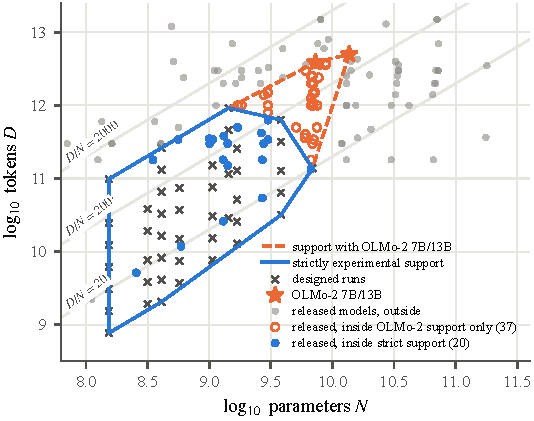
\includegraphics[width=0.75\textwidth]{ra4_obsfix_fig_support}
\caption{Designed Runs, Released Models and the Common Support}\label{fig:support}
\begin{figurenotes}
Log parameters and log training tokens of the designed runs (crosses: the OLMo ladder and \citealp{gadre2024language}
with $N\geq0.1$B) and of the 128 released base models (dots). Solid line: convex hull of the designed runs (the
strictly experimental support; 20 released models inside, filled). Dashed line: hull including the released OLMo-2 7B
and 13B models (stars; 37 more released models inside, open circles). Gray lines: 20, 200 and 2,000 tokens per
parameter.
\end{figurenotes}
\end{figure}

\subsection{Support and Inference}

The strictly experimental support is small (Figure~\ref{fig:support}). Without the released OLMo-2 models, the largest
designed $D$ is 921 billion tokens (one run of \citealp{gadre2024language} at 1.4 billion parameters), and above 3.8
billion parameters it is 634 billion. The strict support contains 20 released models from 9 families and 6
developers, all released between March 2021 and September 2023 with at most 6.7 billion parameters and 627 billion
tokens; five of the nine families have two or more models, 16 models in all. The benchmark that includes OLMo-2 (88
runs) covers 57 models from 30 families and 19 developers, with at most 8.8 billion parameters. Fifteen of its families
have two or more models (42 models) and fifteen are singletons. We report both designs.

Inference must allow for few clusters and for the uncertainty of the benchmark itself. Standard errors are CV3
jackknife standard errors by developer \citep{mackinnon2023cluster}. The benchmark's uncertainty comes from a
design-conditional wild bootstrap of the surface, clustered by design and model size. For each bias we compute three
few-cluster $p$-values that include the benchmark's uncertainty: CV3 with $t(G-1)$ critical values, and restricted
wild-cluster bootstrap-$t$ tests studentized by CR1 or by CV3 \citep{cameron2008bootstrap,webb2023reworking}.
Table~\ref{tab:matched} reports the largest of the three, so a rejection requires all three to reject. The effective
number of clusters \citep{carter2017asymptotic} is 2.5 to 6.7 of 19 on the 57-model design. On the strict design it is
1.2 to 3.8 of 6; there the three procedures disagree by up to a factor of ten, and none is reliable.

\input{tables/matched}

\begin{figure}[tp]
\centering
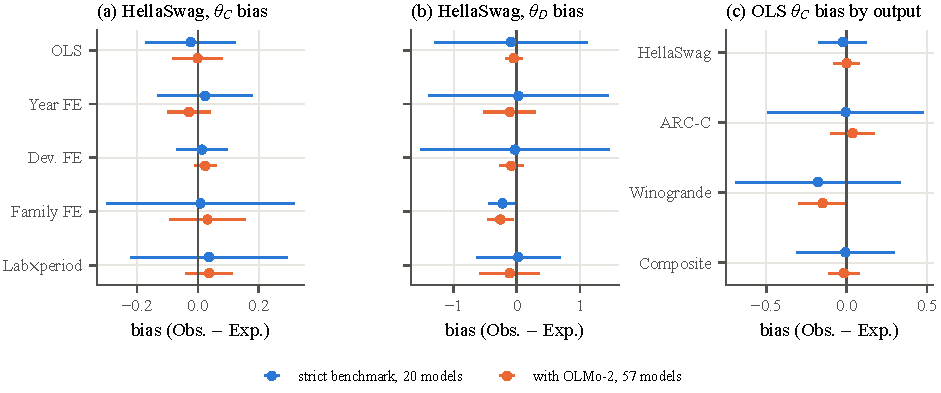
\includegraphics[width=\textwidth]{ra4_obsfix_fig_matched}
\caption{Observational Estimates against the Experimental Technology on the Same Design}\label{fig:matched}
\begin{figurenotes}
Bias of each observational estimator relative to the same estimator applied to the outputs of the experimental
technology on the same models (Obs.\ $-$ Exp.), with 95 percent intervals ($\pm1.96$ CV3 standard errors of the bias,
including the benchmark's uncertainty). Blue: strict benchmark (OLMo ladder and \citealp{gadre2024language}; 20 models).
Orange: benchmark including the released OLMo-2 7B and 13B models (57 models). Panels (a) and (b): HellaSwag,
compute-only elasticity $\theta_C$ and data elasticity $\theta_D$. Panel (c): pooled OLS bias in $\theta_C$ by output;
ARC-Challenge and Winogrande use the censored (Tobit) benchmark. Estimates and conservative few-cluster $p$-values are
in Table~\ref{tab:matched}.
\end{figurenotes}
\end{figure}

\subsection{Returns to Compute}

Once the design is matched, cross-lab returns to compute on HellaSwag do not differ detectably from the experimental
technology (Table~\ref{tab:matched}, Figure~\ref{fig:matched}). On the 57-model design, pooled least squares gives
$\theta_C=0.328$, against 0.329 from the experimental technology on the same models, a bias of $-0.001$ (standard error
0.041) with $p=0.98$. Across six estimators, from pooled least squares to developer-by-period fixed effects and the
notability-propensity control, the biases lie between $-0.029$ and $+0.037$, and every $p$-value is at least 0.36. The
strict surface evaluated on the same 57 models, an extrapolation for 37 of them, gives $+0.014$ (0.045), so the result
does not rest on anchoring the surface with OLMo-2. On the strict support itself the point estimates do not move (from
$-0.024$ to $+0.037$ across five estimators), but with six clusters they carry no inferential weight.

This is a failure to reject in a joint test of low power, not evidence of unbiasedness. On 57 models the 95 percent
interval for the least-squares bias, with $t(18)$ critical values, is $[-0.088,0.086]$, about 26 percent of the
benchmark on either side. The bias detectable with 80 percent power is 0.12, or 37 percent of the benchmark; on the
strict support it is 0.27, or 62 percent. The test covers only models with at most 8.8 billion parameters, and its
benchmark is the technology of the AI2 and OpenLM recipes.

\textit{Other benchmarks.} ARC-Challenge and Winogrande are less informative, because many small designed runs score at
or below chance: 52 of the 86 runs are at the floor of chance-adjusted accuracy on ARC-Challenge and 16 on Winogrande,
against 2 on HellaSwag. A least-squares surface fitted to the clipped log-odds makes the observational compute
elasticity on ARC-Challenge look attenuated, with a bias of $-0.098$ on 57 models. The attenuation does not survive
modeling the censoring. We fit a Tobit surface censored at the floor, match its level to the observed outputs, and clip
the counterfactual at the same floor; the bias is then $+0.036$ (0.069), with $p=0.61$. The Tobit benchmark
extrapolates a Gaussian latent surface below the floor for 60 percent of the runs, so we do not read it as showing that
the attenuation was an artifact. Winogrande keeps a borderline attenuation: $-0.150$ (0.077) on 57 models, with
$p$-values between 0.068 and 0.084 across the three procedures. On the strict support the Winogrande estimate is
similar but uninformative ($-0.179$, $p=0.53$).

Two parts of the joint null are not tested. Observational outputs come from the leaderboard's harness, whereas the
designed runs were evaluated in the OLMES and LLM-foundry harnesses with other prompts and numbers of shots; we
harmonize them only through the log-odds of chance-adjusted accuracy. And benchmark contamination, or
classifier-filtered corpora that favor benchmark-like text \citep{dominguezolmedo2025training}, raise output at given
inputs; family effects absorb such shifts only when they are common to a family.

\subsection{Parameters versus Data}\label{sec:split}

The split between parameters and data is not reliably estimated. With family fixed effects on the 57-model design, the
observational parameter elasticity exceeds the benchmark by 0.203 (0.059) and the data elasticity falls short of it by
0.262 (0.106). The conservative $p$-values are 0.048 and 0.027, and dropping any one developer leaves both signs
unchanged (Appendix Table~\ref{tab:inference}). But the identifying variation is thin. The effective number of clusters
is about 4 of 19, and two families supply 65 percent of the leverage for $\theta_D$: Cerebras-GPT, trained at exactly 20
tokens per parameter, and Phi, trained on synthetic data. Under the strict benchmark the biases have similar size
($+0.185$ and $-0.227$) but conservative $p$-values of 0.14 and 0.15. Biases of opposite sign are also hard to
reconcile with transmission: if wedges are unrelated to productivity at given compute, transmission shifts both
elasticities by the same amount (Section~\ref{sec:transmission}). Opposite signs point instead to factor-biased recipe
changes within families or to errors in $D$, which the benchmark cannot distinguish from bias. We read them as a
within-family disagreement driven by two families, not as a finding.

Both the observational data and the experimental technology agree that $\theta_N>\theta_D$ on this design: 0.42
against 0.27 under the experimental technology on the 57 models, and $\theta_N-\theta_D=0.21$ (0.08) in the
observational data on all 128. Over-trained models have wedges above one, so their output elasticity with respect to
parameters exceeds that with respect to data. A regression on $\ln C=\ln6ND$ alone therefore imposes equal weights
that the data reject, and the residual of such an equal-weight index misattributes
$\tfrac12(\theta_N-\theta_D)(\Delta n-\Delta d)$ to productivity (Corollary~\ref{cor:growth}(iii)): as models shift
further toward tokens, measured productivity understates progress.

\subsection{How Large Could Transmission Bias Be?}\label{sec:matched-size}

Two exercises calibrate the size of the biases that the validation could have missed. In the first, we treat the 25
pretraining recipes of DataDecide as labs with real outcomes and simulate how they choose model size. Pooled least
squares is then unbiased under exogenous budgets. It overstates $\theta_C$ by 0.044 when funding rises with
productivity rank, and understates it by 0.18, or 39 percent, when each lab trains to a common capability target.
Cross-family productivity dispersion in the observational panel is about five times that of the recipes, which scales
the funding bias to about $+0.2$ and the target bias beyond $-0.18$. The 95 percent interval of the matched bias
excludes both. The data are therefore consistent with budgets roughly orthogonal to productivity, or with offsetting
funding and release selection; the simulated rules are stylized.

% Generated by code/paper/make_companion_tables.py from output/tables/m6_montecarlo_industry_summary.csv.
\begin{table}[tp]
\centering
\caption{Production-Function Estimators in a Simulated Industry}
\label{tab:industry}
\footnotesize
\setlength{\tabcolsep}{5pt}
\begin{tabular}{@{}l ccccc@{}}
\toprule
 & \multicolumn{4}{c}{All released models} & Flagships only \\
\cmidrule(lr){2-5}\cmidrule(lr){6-6}
 & (a) & (b) & (c) & (d) & (e) \\
Compute rule: & Exogenous & Funding & Target & Predetermined & Funding \\
\midrule
\multicolumn{6}{@{}l}{\textit{Panel A. Frontier elasticity $\gamma$ (truth 0.178)}} \\
Pooled Huber, $E$ free & 0.019 & 0.027 & $-$0.004 & 0.025 & 0.117 \\
 & [0.031] & [0.036] & [0.022] & [0.035] & [0.123] \\
Pooled NLS, generation effects & $-$0.001 & 0.023 & $-$0.053 & 0.018 & 0.118 \\
 & [0.010] & [0.024] & [0.056] & [0.019] & [0.121] \\
Developer effects & 0.000 & 0.008 & $-$0.022 & 0.004 & 0.113 \\
 & [0.006] & [0.009] & [0.024] & [0.007] & [0.114] \\
Developer $\times$ generation effects & 0.000 & 0.000 & 0.000 & 0.000 & n.a. \\
 & [0.002] & [0.003] & [0.002] & [0.002] &  \\
\addlinespace[3pt]
\multicolumn{6}{@{}l}{\textit{Panel B. Productivity growth per generation (truth 0.150)}} \\
Pooled Huber, $E$ free & $-$0.081 & $-$0.090 & $-$0.036 & $-$0.088 & $-$0.145 \\
 & [0.081] & [0.090] & [0.039] & [0.088] & [0.146] \\
Pooled NLS, generation effects & 0.002 & $-$0.024 & 0.054 & $-$0.018 & $-$0.130 \\
 & [0.012] & [0.027] & [0.055] & [0.021] & [0.132] \\
Developer effects & 0.001 & $-$0.009 & 0.023 & $-$0.003 & $-$0.124 \\
 & [0.010] & [0.013] & [0.025] & [0.010] & [0.125] \\
Developer $\times$ generation effects & 0.001 & 0.000 & 0.000 & 0.001 & n.a. \\
 & [0.009] & [0.009] & [0.009] & [0.009] &  \\
\bottomrule
\end{tabular}
\par\smallskip
\begin{tablenotes}Bias [root-mean-squared error] over 400 replications per column. Forty developers each produce six generations of models and release one to four models per generation, about eightfold apart in compute; productivity is Hicks-neutral, $\omega_{ft}=0.15(t-1)+x_{ft}$ with $x_{ft}$ a persistent AR(1) (coefficient 0.8, standard deviation 0.25). Compute rules: (a) exogenous budgets; (b) funding, log compute rises by $2x_{ft}$; (c) a common loss target reached by buying compute; (d) predetermined budgets, log compute rises by $2x_{f,t-1}$; (e) rule (b) with one model per developer and generation. Allocations include inference demand (mean log wedge 0.46) and allocation errors (standard deviation 0.2 in $\ln(D/N)$). The pooled Huber fit estimates $E$ and has no time effects, as is common in machine-learning practice; the other estimators know $E$. Developer $\times$ generation fixed effects use only the menu of sizes within a developer's generation and are not defined with flagships only (n.a.). Productivity growth: mean change in generation means of $y-\hat F(n,d)$. Every estimator starts from data-based values. The calibration is illustrative; magnitudes scale with the assumed share of productivity-driven variation in compute. Appendix Table~\ref{tab:industry-full} reports all estimators and parameters.\end{tablenotes}
\begin{tablenotes}[Source]Author's simulations; replication code \texttt{code/analysis/m6\_montecarlo} (entry point \texttt{run\_v2.py}).\end{tablenotes}
\end{table}


The second exercise is a simulated industry in which the compute rule is known (Table~\ref{tab:industry}; the design
and all estimators are in Appendix~\ref{app:mc}). Forty developers each produce six generations of models, release one
to four models per generation, and choose compute by one of four rules. Pooled nonlinear least squares with generation effects overstates $\gamma$ by 13 percent under
funding and understates it by 30 percent under a capability target. With one flagship per developer and generation,
the overstatement under funding is 66 percent, as Proposition~\ref{prop:transmission}(i) predicts for one model per
lab. Developer fixed effects remove about two-thirds of the funding bias but little of it with flagships only, because
productivity is persistent rather than fixed. Estimation within developer and generation, the observational analog of
an IsoFLOP sweep, is unbiased under every rule, but it requires at least two released siblings. The specification most
common in machine learning, a pooled fit with $E$ free and no time effects, misses more than half of productivity
growth under three of the four rules, mostly by attributing it to scale (Corollary~\ref{cor:growth}(ii)) and partly
to a downward-biased estimate of $E$. The calibration is illustrative; only signs and rankings should be read from
it.

% =====================================================================================================================
\section{Measurement of Compute and the Standard Remedies}\label{sec:compute}

\textit{Measurement error.} Measurement error in compute is small, but showing it requires an independent measure.
Compute in the panel is $C=6ND$ from reported $N$ and $D$, and Epoch's compute figures for these models are mostly
$6ND$ itself (operation counting) or developer-reported counts of the same kind. Only records of hardware time measure
compute independently of the reported inputs. We rebuild compute from them as chip-hours times peak dense 16-bit
throughput times a common utilization of 0.3. We do not use Epoch's utilization field, which is back-calculated from
Epoch's own compute estimate in every record we checked. Across the 27 models with such records, from 12 families,
$\ln(C_{\rm hw}/6ND)$ has a standard deviation of 0.29, with 95 percent interval $[0.20,0.41]$ (Appendix
Table~\ref{tab:reliability}). This bounds the error in
$\ln6ND$ from above, because it also contains differences in true utilization and errors in chip-hours. The implied
reliability of $\ln C$ on the 57-model design is at least 0.98 pooled and 0.955 within families. Correcting for errors
in variables raises the pooled compute elasticity by 0.007 and the within-family elasticity by 0.021, or by 0.042 at
the upper end of the interval for the error standard deviation (Appendix Table~\ref{tab:compute}).\footnote{An earlier
version of this analysis reported a within-family errors-in-variables estimate of 0.858 against a benchmark of 0.409.
It used Epoch's `Confident' uncertainty class ($\sigma_u=\ln3/1.645=0.67$), which describes the uncertainty of Epoch's
own estimate rather than the error in $6ND$, and it computed the within-family variance of $\ln C$ with an $n-1$
denominator, ignoring the 30 family means. With the correct variance and the hardware-time bound, the within-family
bias is $+0.052$ (0.049), with $p=0.30$.}

\textit{Reverse regression.} The reverse regression of $\ln C$ on output gives an inverse slope of 0.560. By
construction this equals the forward slope, 0.328, divided by the forward $R^2$ of 0.585 (with family effects,
$0.441/0.760=0.580$). Its distance from the same statistic computed on the experimental outputs, 0.352, therefore
measures output variation not explained by compute (productivity dispersion and noise), not a bias. Under funding,
the forward--reverse pair need not bracket the truth at all (Proposition~\ref{prop:transmission}(iii)).

\textit{Instruments, panels and proxies.} The standard remedies for transmission bias cannot be used, for reasons that
concern the data rather than the estimators. The price-performance of the best available data-center accelerator is a
step function of calendar time. On the 57-model design its first-stage $F$ is 0.90 (0.01 with developer fixed effects),
and the Anderson--Rubin sets are unbounded. Applied to the experimental outputs, the same instrument recovers 0.012
against a design-matched elasticity of 0.33: the instrument fails, not the data. The price-performance of each model's
own training hardware is strong only on 10 models from 7 developers ($F=14.3$), and it takes three values, so it acts
as an indicator of vintage; its Anderson--Rubin set is $[-1.50,0.34]$. An export-control instrument (Chinese developers
after October 2023, with developer and year effects) is strong among the 90 models with at most 14 billion parameters
and 5 trillion tokens ($F=10.6$). It gives $\theta_C=0.90$ (0.25), with Anderson--Rubin set $[0.49,2.23]$, which is 1.7
to 2.3 times the least-squares and fixed-effects estimates on that sample. Its exclusion restriction fails because
recipes and data changed at the same time. Dynamic-panel estimators \citep{arellano1991some,blundell1998initial} need
three consecutive generations of a product line, which only six product-line cells have. Proxy inversion is unavailable
for the reasons of Proposition~\ref{prop:proxy}. The notability-propensity control barely moves the matched bias
($-0.015$, $p=0.80$).

% =====================================================================================================================
\section{Productivity Dispersion}\label{sec:tfp}

How dispersed is productivity across model families? The answer depends on the units in which it is measured
(Table~\ref{tab:tfp}). Let $\Delta$ be the gap between the 90th and 10th percentiles of family productivity in
HellaSwag log-odds, net of inputs. In output units the 90--10 ratio of the odds, $e^{\Delta}$, is 1.9 to 3.0 across
samples and netting methods. In reducible-loss units, $e^{\gamma\Delta/\theta_C}$ with the frontier elasticity
$\gamma=0.178$ of \citet{besiroglu2024chinchilla}, it is 1.3 to 1.8. The 90--10 ratio within US manufacturing
industries, 1.92 \citep{syverson2004product}, lies at the bottom of the first range and just above the second. In compute-equivalent units, $e^{\Delta/\theta_C}$,
the compute that the 10th-percentile family needs to match the 90th, the ratio is 7 to 24 with the 57-model benchmark
$\theta_C=0.33$, or 4 to 13 with the strict benchmark's 0.43. Within developers, in the design of
\citet{mertens2026secret}, it is 11.1 in compute units, against their 41 on another benchmark.

Manufacturing's ratio is both an output-unit and an input-unit ratio, because returns to scale are near one. For
language models the two differ by the factor $1/\theta_C$ in logs, between 2.3 and 3, because returns to compute are
small. The comparison with manufacturing is therefore a choice of cardinalization, not a finding.

\begin{table}[tp]
\centering
\caption{Productivity Dispersion across Model Families in Output and Input Units}
\label{tab:tfp}
\footnotesize
\setlength{\tabcolsep}{3pt}
\begin{tabular}{@{}l cccccc@{}}
\toprule
 & Output units & Compute & Loss & Compute & Loss &  \\
 & odds & \multicolumn{2}{c}{$\theta_C=0.33^{a}$} & \multicolumn{2}{c}{$\theta_C=0.43$} & $\theta$ used \\
\cmidrule(lr){3-4}\cmidrule(lr){5-6}
 & (1) & (2) & (3) & (4) & (5) & (6) \\
\midrule
\multicolumn{7}{@{}l}{\textit{All 128 models (38 families)}} \\
Family effects, $\theta_C$ netting & 2.68 & 19.9 & 1.70 & 13.1 & 1.58 & 0.33 \\
 & $[1.94,5.27]$ & $[7.5,160.7]$ & $[1.43,2.47]$ & $[5.1,69.8]$ & $[1.34,2.13]$ &  \\
Family effects, within netting & 2.83 & 23.7 & 1.76 & 11.2 & 1.54 & 0.33 \\
 & $[2.02,5.59]$ & $[8.5,193.1]$ & $[1.46,2.56]$ & $[5.1,53.7]$ & $[1.34,2.03]$ &  \\
Within-developer residuals & 2.78 & 11.1 & 1.54 &  &  & 0.43 \\
 & $[1.77,3.19]$ & $[4.1,18.1]$ & $[1.29,1.68]$ &  &  &  \\
\addlinespace[2pt]
\multicolumn{7}{@{}l}{\textit{Without distilled and synthetic-data models}} \\
Family effects, $\theta_C$ netting & 2.57 & 17.6 & 1.67 & 13.1 & 1.58 & 0.33 \\
 & $[1.90,5.13]$ & $[7.0,143.9]$ & $[1.42,2.43]$ & $[5.1,58.9]$ & $[1.34,2.07]$ &  \\
Family effects, within netting & 2.60 & 18.3 & 1.68 & 9.2 & 1.49 & 0.33 \\
 & $[1.87,5.90]$ & $[6.8,216.6]$ & $[1.41,2.61]$ & $[4.3,58.9]$ & $[1.30,2.07]$ &  \\
Within-developer residuals & 2.84 & 11.3 & 1.54 &  &  & 0.43 \\
 & $[1.78,3.21]$ & $[4.0,18.0]$ & $[1.28,1.67]$ &  &  &  \\
\addlinespace[2pt]
\multicolumn{7}{@{}l}{\textit{Also without code families (32 families)}} \\
Family effects, $\theta_C$ netting & 2.07 & 9.1 & 1.48 & 6.9 & 1.41 & 0.33 \\
 & $[1.70,2.29]$ & $[4.9,12.7]$ & $[1.33,1.57]$ & $[3.5,10.4]$ & $[1.25,1.52]$ &  \\
Family effects, within netting & 1.90 & 7.0 & 1.41 & 4.4 & 1.30 & 0.33 \\
 & $[1.61,5.10]$ & $[4.2,143.4]$ & $[1.29,2.42]$ & $[3.3,37.3]$ & $[1.23,1.91]$ &  \\
Within-developer residuals & 2.51 & 8.4 & 1.46 &  &  & 0.43 \\
 & $[1.71,3.04]$ & $[3.8,14.2]$ & $[1.27,1.61]$ &  &  &  \\
\addlinespace[2pt]
Manufacturing \citep{syverson2004product} & 1.92 & 1.92 & 1.92 & 1.92 & 1.92 & $\approx1$ \\
\bottomrule
\end{tabular}

\begin{tablenotes}
90--10 ratios of Hicks-neutral productivity on HellaSwag log-odds $q$. A gap $\Delta$ between the 90th and 10th percentiles is reported as an odds ratio $e^{\Delta}$ (column 1, output units), as compute-equivalents $e^{\Delta/\theta_C}$ (input units: the compute the 10th-percentile family needs to match the 90th), and in reducible-loss units $e^{\gamma\Delta/\theta_C}$ with $\gamma=0.178$ \citep{besiroglu2024chinchilla}; $\gamma=0.155$ \citep{hoffmann2022training} is in the replication files. $\theta_C=0.33$: the design-matched benchmark on 57 models (benchmark including OLMo-2); $\theta_C=0.43$: the strictly experimental benchmark on 20 models (Table~\ref{tab:matched}). Family effects net inputs either with the benchmark $\theta_C$ or with the within-family $(\theta_N,\theta_D)$; within-developer residuals follow \citet{mertens2026secret} (developer and year effects, single-model developers dropped) and use the regression's own $\theta_C$ (column 6) in columns 2--3 ($^{a}$). Brackets: 90 percent intervals from a developer-cluster bootstrap (999 draws) that also draws $\theta_C$ from its benchmark bootstrap. Manufacturing's 1.92 is an output-unit ratio and, with returns to scale near one, also an input-equivalent ratio; for LLMs the two differ by the factor $1/\theta_C$ in logs, because returns to compute are small. Family effects also absorb benchmark contamination, similarity of training data to the benchmark and omitted teacher compute (distillation, synthetic data).
\end{tablenotes}
\begin{tablenotes}[Source]
Author's calculations; outputs from \citet{ruan2024observational} and \citet{maiapolo2024sloth}.
\end{tablenotes}
\end{table}


Three caveats apply. First, family effects absorb benchmark contamination and the similarity of training data to the
benchmark, as well as productivity. Second, training compute omits the compute of teachers and synthetic-data
generators. With inputs netted within families, the synthetic-data families Phi and SmolLM rank first and third of 38,
so measured productivity credits the student with an intermediate input, the gross-output problem of
\citet{gandhi2020identification}. Third, the conversion to compute rests on a single cardinal elasticity from one
benchmark; the intervals in Table~\ref{tab:tfp} draw $\theta_C$ from its bootstrap. Transmission, finally, would make
all of these ratios understate dispersion (Proposition~\ref{prop:transmission}(ii)).

% =====================================================================================================================
\section{Algorithmic Progress}\label{sec:progress}

\citet{ho2024algorithmic} estimate that the compute needed to reach a given perplexity halves every 8.4 months. Their
data and code are public, and their preferred model is the technology \eqref{eq:tech} with $E=0$, $\kappa=1$ and
factor-augmenting productivity growing linearly in time, $\psi_N=g_Nt$ and $\psi_D=g_Dt$:
\[
\ln\text{ppl}=\exp(\alpha_{0b}-\alpha g_Nt-\alpha\ln N)+\exp(\beta_{0b}-\beta g_Dt-\beta\ln D),
\]
where $b$ indexes three benchmarks and $t$ is time in years. Effective compute grows at $g_C=g_N+g_D$ per year and
doubles every $\tau_C=12\ln2/g_C$ months; Hicks neutrality is $\alpha g_N=\beta g_D$. Their appendix plots the joint
bootstrap distribution of the two year coefficients; we ask what its shape implies for the doubling time.

\subsection{The Ridge}

The rate is weakly identified because the sample is not on the expansion path, a problem of the kind studied by
\citet{diamond1978measurement}. To first order the data pin down how fast loss falls at fixed inputs, an average of
$\alpha g_N$ and $\beta g_D$ weighted by the mean shares of the two terms in loss (0.55 and 0.45). The doubling time
instead weights the two rates by $1/\alpha$ and $1/\beta$. The two combinations coincide only on the expansion path,
along which parameters would grow with compute at elasticity $a=0.37$ under their exponents. Off the path, pairs of
rates that fit equally well imply different doubling times.

Figure~\ref{fig:ridge} shows the resulting ridge. The bootstrap correlation between $\alpha g_N$ and $\beta g_D$ is
$-0.73$ with the authors' code and $-0.82$ at the converged estimates discussed below. The profile-likelihood interval
for $\tau_C$ is $[4.1,40.5]$ months. The parameter-augmenting share $g_N/g_C$ can lie anywhere in $[-0.44,3.37]$ (95
percent profile interval), and over that range $\tau_C$ runs from 5.3 to 39.6 months (Table~\ref{tab:progress}). These
likelihood ratios assume independent Gaussian errors, although observations are clustered by paper. The profile over
$g_N/g_C$ also has a second local minimum near $-0.28$; a missed global minimum could only widen the interval.

\begin{figure}[tp]
\centering
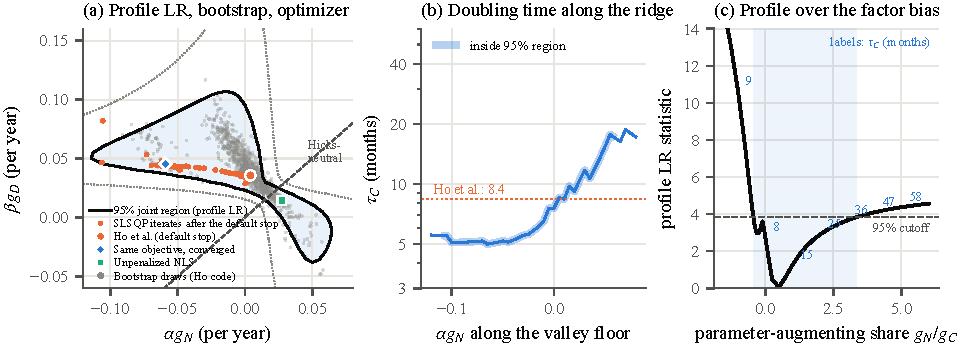
\includegraphics[width=\textwidth]{appE_ridge}
\caption{The Ridge in Estimates of Algorithmic Progress}\label{fig:ridge}
\begin{figurenotes}
Data of \citet{ho2024algorithmic}, 231 model--benchmark observations. Panel (a): 95 percent joint profile-likelihood
region for the year terms $(\alpha g_N,\beta g_D)$, bootstrap draws from the authors' code, the optimizer's iterates
from its default stopping point to the converged minimum of the same objective, the unpenalized least-squares minimum,
and the Hicks-neutral line. Panel (b): doubling time of effective compute $\tau_C$ along the floor of the profile; the
thick segment lies inside the 95 percent region. Panel (c): profile likelihood-ratio statistic over the
parameter-augmenting share $g_N/g_C$, with the implied $\tau_C$ in months at selected points; the dashed line is the 95
percent cutoff and the shaded band the 95 percent interval, $[-0.44,3.37]$. Likelihood ratios assume independent
Gaussian errors.
\end{figurenotes}
\end{figure}

\subsection{Neutrality}

Precision about the rate is bought with an assumption about the bias. Hicks neutrality is not rejected (bootstrap
$p=0.29$ and 0.94 for the converged penalized and the unpenalized estimators), which reflects low power rather than
evidence of neutrality. Imposing it gives 9.2 months with unpenalized least squares, with interval $[6.3,14.3]$, or 11.6
months with the converged penalized estimator: the tightest intervals among the specifications that the data do not
reject. As \citet{diamond1978measurement} predict, the rate is identified here by the restriction on the bias. Even
that restriction is fragile. If the true technology has $E>0$, neutrality imposed within the $E=0$ form is
misspecified. In simulations on Ho et al.'s design with a true doubling time of 12 months, it yields 4.2 to 4.4 months,
so the neutral estimates may overstate progress.

\input{tables/progress}

\subsection{Replication and the Published Estimate}

We reproduce Ho et al.'s estimates exactly from their data and code: the same value of their objective (0.0518), every
parameter within $4\times10^{-7}$, and a bootstrap median of 8.44 months under their protocol
(Table~\ref{tab:progress}, Panel~A). The published 8.4 months is that median; the point estimate is 8.7. The estimator
minimizes mean squared error plus an $L_1$ penalty, using SciPy's SLSQP routine with its default stopping rule, which
halts after 18 iterations. On a flat ridge this setting matters. Run to convergence from the same start, the objective
falls from 0.0518 to 0.0507 while mean squared error changes by only 0.27 percent, and all 300 random starts end below
the published value. Almost all of the improvement comes from the penalty, on constants whose values depend on an
arbitrary normalization. The converged point has $\tau_C=6.1$ months, with a paper-cluster interval of $[3.0,22.7]$,
about twice as wide as published. Unpenalized least squares gives 10.2 months, with interval $[4.1,27.6]$. Estimators of
the same model thus give 6.1 to 10.2 months, and the data cannot arbitrate between them. We read this as a consequence
of the ridge, not as a correction of the published rate: on a flat objective, the stopping rule and the penalty select
the point. The finding concerns numerical optimization, not the order of magnitude of progress: every point estimate of this
model lies between half a year and a year per doubling. It parallels the finding of \citet{besiroglu2024chinchilla} for the
third approach of \citet{hoffmann2022training}, and convergence problems familiar from demand estimation
\citep{dube2012improving,knittel2014estimation}.

\subsection{Why Is the Data Exponent Small?}

Ho et al.'s data exponent is 0.04, against about 0.37 in experiments, and \citet{whitfill2025note} reads the gap as
evidence that progress is overstated about ninefold: dividing their year coefficients by experimental exponents gives
76.5 months. Imposing experimental exponents in estimation is rejected (mean squared error rises by a factor of 1.3 to
4.8 across 14 experimental technologies) and implies negative or implausibly slow progress. Two specification choices
explain much of the exponent gap while moving $\tau_C$ much less (Appendix Table~\ref{tab:attenuation}). First, fitting
the $E=0$ form to the Chinchilla sweep itself lowers the frontier elasticity from 0.178 to 0.053, close to the sweep's
mean elasticity of total rather than reducible loss (0.054). The like-for-like gap is therefore about 2 to 2.5-fold,
not 7 to 9-fold. Dropping $E$ rescales exponents and year coefficients by similar factors, so rates barely move:
imposing a common $E$ from 0 to 1.5 nats per word doubles $\hat\gamma$ but moves $\tau_C$ only from 10.2 to 12.4
months. Ho et al.'s data themselves prefer $E=0$ within this form, so this argument rests on the sweep and on
simulations; in the simulations the authors' procedure can also stop at a local optimum that overstates progress.
Second, their $D$ is dataset size, while small models were trained for a median of 62 to 140 epochs. Measuring
effective data under repetition \citep{muennighoff2023scaling} raises $\tau_C$ by a factor of 1.5 to 4, with an
unbounded upper confidence limit.

\subsection{Scale Dependence and Frontier Regressions}

Two further questions need designed data. Whether the compute-equivalent gain of transformers over earlier
architectures depends on scale turns on whether their frontier elasticities differ (Corollary~\ref{cor:growth}(i)). In
Ho et al.'s data the difference is 0.008, with interval $[-0.012,0.034]$, and bootstrap intervals for the implied gains
span six orders of magnitude (Appendix Table~\ref{tab:ceg-sahal}). And regressions of loss on compute that omit time
effects overstate the compute elasticity by a factor of 1.15 on all 231 observations and 1.44 among 36 record-setting
releases (Corollary~\ref{cor:growth}(ii)). Among record setters, whose compute moves closely with time, independently
measured growth rates imply an algorithmic share of 0.37 and a predicted factor of 1.58, consistent with the estimate.
On all observations the prediction fails, because compute and time are only moderately correlated (0.62), and the
ordinary omitted-variable formula applies instead.

\subsection{The Missing Data}

Proposition~\ref{prop:dmr} names the data that would settle these questions: IsoFLOP sweeps at several vintages on a
common output, whose drift in the compute-optimal $M^*$ signs the bias of technical change and whose curvature fixes
its size. The controlled experiment of \citet{okar2026what} supplies the cross-sectional analog for a change in data
quality at one date.
\textcolor{red}{[TBD-m9: one sentence on the shift in the compute-optimal $M^*$ at fixed compute between the two
corpora of the experiment, and hence the sign of the Hicks bias of the data-quality difference
(Proposition~\ref{prop:dmr}(i) applied across corpora rather than dates); delete if m9 cannot answer it.]}

% =====================================================================================================================
\section{Allocative versus Technical Change}\label{sec:allocative}

Measured progress, the fall in the compute needed to reach a given loss, mixes shifts of the frontier with movements
toward it. By Proposition~\ref{prop:farrell}, the move from Kaplan-rule to Chinchilla-rule allocations changed the mix,
not the technology, so its gain is allocative. \citet{gundlach2025origin} define the compute-equivalent gain from such
rebalancing and count it as algorithmic progress.

\textit{Measurement.} Measuring the gain realized between eras requires a choice. Training-cost efficiency, the
Farrell efficiency against the training-only frontier \citep{farrell1957measurement}, $C_{\min}(L(N,D))/6ND$, counts
deliberate over-training as waste, although over-training reflects the value that labs place on compact models.
Serving demand cannot produce a wedge below one (Section~\ref{sec:tech}). We therefore count only the elimination of
under-training: training-cost efficiency evaluated at $\min(w,1)$, which by Lemma~\ref{lem:alloc}(iii) depends on the
wedge alone. The truncated measure attributes every wedge below one to allocative error. A wedge below one can also
reveal a binding data constraint or data-augmenting productivity specific to the lab. For 2020--21 models trained on a
few hundred billion tokens, a belief in the law of \citet{kaplan2020scaling} is the more plausible reading, but it
remains an assumption.

\textit{Realized gains.} We compare models in the Epoch database with at least $10^{23}$ FLOP: 7 released in 2020--21
(era 1) and 92 in 2022--24 (era 2) (Table~\ref{tab:allocative}, Figure~\ref{fig:allocative}). Every era-1 model has
$w<1$ under every technology, and the median ratio of tokens to parameters rose from 1.7 to 92 between the eras.
Counting only the elimination of under-training, geometric-mean training-cost efficiency rose by a factor of 2.0 under
the reference technology of \citet{okar2026what} (Chinchilla with $\kappa$ free) and 1.7 under
\citet{besiroglu2024chinchilla}, with 95 percent interval $[1.21,2.44]$. Across all 14 estimated technologies the factor
ranges from 1.1 to 4.9. Era-2 releases closed 80 to 94 percent of the era-1 under-training gap, in logs. The positive
sign is close to mechanical, because every era-1 model is under-trained and truncation can only raise era-2 efficiency;
the content is in the size. Without truncation the gain ranges from 0.55 to 4.3 across technologies: counting
over-training as waste can reverse its sign.

\begin{table}[tp]
\centering
\caption{Allocative Gains from Rebalancing, with and without Truncating the Wedge at One}
\label{tab:allocative}
\footnotesize
\setlength{\tabcolsep}{2.6pt}
\begin{tabular}{@{}l c cc cc cc@{}}
\toprule
 & $w<1$ (\%) & \multicolumn{2}{c}{Untruncated} & \multicolumn{2}{c}{Truncated} & Gap & Kaplan \\
\cmidrule(lr){3-4}\cmidrule(lr){5-6}
 & era 1/2 & Gain & 95\% CI & Gain & 95\% CI & closed & CEG \\
 & (1) & (2) & (3) & (4) & (5) & (6) & (7) \\
\midrule
\multicolumn{8}{@{}l}{\textit{Chinchilla sweep}} \\
\citet{besiroglu2024chinchilla} & 100 / 18 & 1.05 & $[0.57,1.75]$ & 1.68 & $[1.21,2.44]$ & 0.92 & 11.7 \\
\citet{hoffmann2022training} & 100 / 45 & 1.91 & $[1.53,2.50]$ & 2.34 & $[1.87,3.03]$ & 0.88 & 32.4 \\
\citet{hoffmann2022training}, rounded & 100 / 50 & 2.41 & $[1.86,3.24]$ & 2.77 & $[2.16,3.69]$ & 0.86 & 46.7 \\
Chinchilla, $\kappa$ free (reference) & 100 / 26 & 1.19 & $[0.92,1.56]$ & 1.97 & $[1.58,2.53]$ & 0.92 & 20.3 \\
\multicolumn{8}{@{}l}{\textit{Other public sweeps, Chinchilla form \citep{okar2026what}}} \\
Farseer, total $N$ & 100 / 42 & 1.58 & $[1.27,2.04]$ & 2.06 & $[1.66,2.60]$ & 0.89 & 38.7 \\
Farseer, non-embedding $N$ & 100 / 18 & 1.03 & $[0.86,1.25]$ & 1.54 & $[1.32,1.84]$ & 0.92 & 7.3 \\
\citet{gadre2024language}, C4 & 100 / 12 & 0.60 & $[0.51,0.70]$ & 1.14 & $[1.06,1.26]$ & 0.94 & 3.5 \\
OLMo ladder & 100 / 66 & 2.52 & $[1.99,3.20]$ & 2.63 & $[2.07,3.33]$ & 0.81 & 57.0 \\
\citet{muennighoff2023scaling} & 100 / 38 & 1.74 & $[1.38,2.27]$ & 2.33 & $[1.87,2.97]$ & 0.90 & 18.1 \\
\multicolumn{8}{@{}l}{\textit{Laboratory IsoFLOP designs, Chinchilla form \citep[Online Appendix]{okar2026what}}} \\
Llama 3 IsoFLOPs (Meta) & 100 / 12 & 0.74 & $[0.62,0.90]$ & 1.30 & $[1.16,1.50]$ & 0.93 & 5.1 \\
Marin, Comma & 100 / 62 & 4.31 & $[2.95,6.60]$ & 4.95 & $[3.42,7.50]$ & 0.80 & 388.5 \\
Marin, DCLM & 100 / 50 & 3.04 & $[2.09,4.45]$ & 4.00 & $[2.83,5.77]$ & 0.85 & 230.7 \\
Marin, Nemotron-CC & 100 / 49 & 2.57 & $[1.87,3.68]$ & 3.52 & $[2.55,5.11]$ & 0.86 & 166.3 \\
(Mis)Fitting, FineWeb/C4 & 100 / 12 & 0.55 & $[0.40,0.75]$ & 1.64 & $[1.31,2.12]$ & 0.93 & 15.0 \\
\multicolumn{8}{@{}l}{\textit{Cross-lab regression}} \\
\citet{ho2024algorithmic}, model 7 & 0 / 0 & 0.09 & $[0.07,0.12]$ & 1.00 & $[1.00,1.00]$ & -- & -- \\
\addlinespace[3pt]
\multicolumn{8}{@{}l}{\textit{Other samples, \citet{besiroglu2024chinchilla} technology}} \\
$C\geq10^{23}$, cleaned (7, 79) & 100 / 19 & 1.09 & $[0.60,1.78]$ & 1.70 & $[1.23,2.43]$ & 0.94 &  \\
Top five per year (10, 15) & 70 / 40 & 1.27 & $[0.91,1.72]$ & 1.31 & $[1.05,1.76]$ & 0.73 &  \\
Epoch frontier models (7, 6) & 86 / 33 & 1.56 & $[1.07,2.19]$ & 1.54 & $[1.12,2.19]$ & 0.82 &  \\
\bottomrule
\end{tabular}

\begin{tablenotes}
Models in the Epoch database with $C\geq10^{23}$ FLOP: 7 released in 2020--21 (era 1) and 92 in 2022--24 (era 2); dense, at most four epochs, $D=C/6N$. Training-cost efficiency, the Farrell efficiency against the training-only frontier, $CE=C_{\min}(L(N,D))/6ND$, depends only on the wedge $w=\varepsilon_N/\varepsilon_D$ within the Chinchilla family. Untruncated gain: ratio of era geometric means of $CE$. Truncated gain: the same with $CE(\min(w,1))$, which counts only the elimination of under-training: over-training ($w>1$) can reflect the value of compactness, including serving demand, and is not treated as inefficiency, whereas serving demand cannot produce $w<1$ (\citealp{okar2026what}, Proposition 1). Column 1: share of models with $w<1$. Column 6: $\ln(\text{truncated gain})$ divided by the era-1 log compute lost to under-training. Column 7: compute-equivalent gain of abandoning the Kaplan rule ($N\propto C^{0.73}$ from GPT-3) at $5\times10^{26}$ FLOP, the counterfactual of \citet{gundlach2025origin}; the Kaplan allocations have $w<1$ under every technology, so truncation does not change it. Intervals: percentile bootstrap over models within era (999 draws); only the \citet{besiroglu2024chinchilla} row also draws the technology's parameters, so the other intervals hold the technology fixed, and with seven era-1 models all intervals are rough. A wedge below one is counted as allocative error; by \citet[Proposition 1]{okar2026what} it can also reflect a binding data constraint or data-augmenting productivity specific to the developer. Technologies from other sweeps use each sweep's own $N$ and $D$ conventions and loss corpus, so their levels are indicative. Group labels give the data on which each technology is estimated: the Chinchilla sweep (the reference technology of \citealp{okar2026what} is Chinchilla with $\kappa$ free), Chinchilla-form fits to the other public sweeps and to laboratory IsoFLOP designs, and Ho et al.'s cross-lab model, under which every model has $w>1$.
\end{tablenotes}
\begin{tablenotes}[Source]
Author's calculations from the Epoch AI models database \citep{epochai2026data}.
\end{tablenotes}
\end{table}


\begin{figure}[tp]
\centering
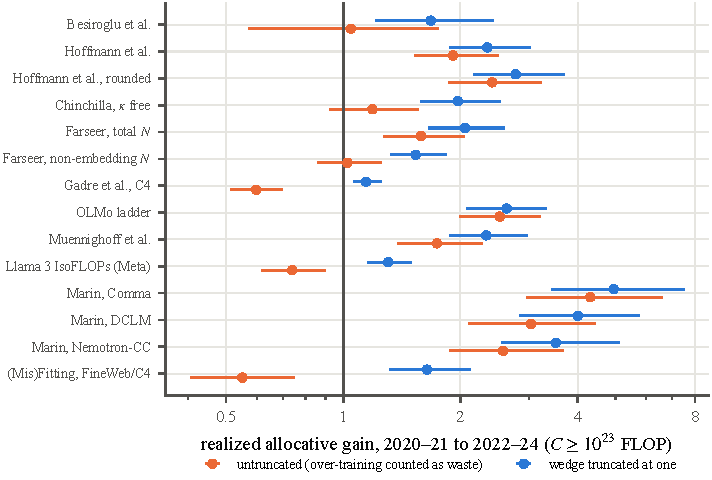
\includegraphics[width=0.85\textwidth]{ra4_obsfix_fig_allocative}
\caption{Realized Allocative Gains from Rebalancing, by Technology}\label{fig:allocative}
\begin{figurenotes}
Ratio of geometric-mean training-cost efficiency, 2022--24 against 2020--21, for Epoch models with at least $10^{23}$
FLOP (7 and 92 models), under each technology, with 95 percent percentile-bootstrap intervals over models within era
(log scale). Orange: efficiency against the training-only frontier, which counts over-training as waste. Blue: the
wedge truncated at one, which counts only the elimination of under-training. Only the \citet{besiroglu2024chinchilla}
interval also reflects uncertainty in the technology's parameters. Estimates in Table~\ref{tab:allocative}.
\end{figurenotes}
\end{figure}

The intervals resample models within era; only the Besiroglu interval also draws the technology's parameters, and with
seven era-1 models all intervals are rough. Technologies estimated on other sweeps use their own conventions for $N$,
$D$ and the loss corpus, so their levels are indicative. The Marin fits, whose parameter exponents are about twice
Chinchilla's, give the largest gains (3.5 to 4.9). Samples of the five largest models per year and of Epoch's frontier
models give smaller and noisier truncated gains (1.3 and 1.5 under Besiroglu).

\textit{Comparison with progress.} Against the effective-compute gain implied by Ho et al.'s published rate over the
same interval, 8.9-fold over 2.28 years, the realized allocative gain amounts to 6 to 73 percent in logs across
technologies (31 percent under the reference technology). The denominator itself ranges from 6.4 to 22.5 across the
estimators of Section~\ref{sec:progress}. \citet{gundlach2025origin} report that the Kaplan-to-Chinchilla rebalancing
is worth about a factor of 10 at the 2025 frontier, and our counterfactual agrees. Under the Besiroglu technology,
continuing Kaplan's rule from GPT-3 would cost a factor of 1.6 at GPT-3's compute, 5.2 at $3.8\times10^{25}$ FLOP and
11.7 at $5\times10^{26}$ FLOP. Because Kaplan-rule allocations have $w<1$ under every technology, truncation does not
affect this counterfactual. What we add is the contrast with the gain realized between eras, 1.1 to 4.9, which is
smaller. Under Ho et al.'s own exponents, finally, every model has $w>1$. An attenuated data exponent makes tokens
nearly worthless, so a regression with those exponents cannot credit rebalancing to inputs and loads it onto the time
trend.

% =====================================================================================================================
\section{Conclusion}\label{sec:conclusion}

Observational data on language models deliver returns to compute once the design is matched, though only as a failure
to reject in a test of low power, and measures of productivity dispersion whose size depends on the units. They do not
deliver the split between parameters and data, the bias of technical change, or its rate without a restriction on the
bias. In each case the missing variation is the variation transverse to the expansion path that designed IsoFLOP
sweeps supply: at given compute, labs choose the mix, and productivity does not move it.

Three implications follow for economists who use these numbers. First, cross-lab regressions of benchmark scores on
compute can be used for returns to compute once the design is matched to an experimental benchmark, but not for the
relative value of parameters and data. Second, headline rates of algorithmic progress from observational
data carry the precision of an identifying assumption about the bias of technical change; forecasts and growth
accounts that use them should carry intervals that span that assumption. Third, rebalancing gains realized in the past
are small relative to counterfactual gains at today's scale, so the importance of allocation for measured progress
depends on which of the two a question needs.

What would settle these questions is designed variation published by labs: IsoFLOP sweeps at several dates on a common
output, and model-level records of hardware time. Both cost little relative to the frontier runs they would
inform, and the second is already partly public. A final lesson is methodological. The industry allows an economist to check
production-function estimators against experiments, and the check works only after the design is matched; where
experiments exist in other industries, the same discipline applies.

\bibliographystyle{aea}
\bibliography{references}

% =====================================================================================================================
\clearpage
\appendix
\makeatletter\renewcommand\p@subsection{}\makeatother
\renewcommand{\theHtable}{\thetable}\renewcommand{\theHfigure}{\thefigure}\renewcommand{\theHequation}{\theequation}

\section[Proofs]{Appendix \thesection. Proofs}\label{app:proofs}

\textit{Proof of Lemma~\ref{lem:alloc}.} (i) Write effective inputs $\tilde n=n+\psi_N$ and $\tilde d=d+\psi_D$,
$u=Ae^{-\alpha\tilde n}$ and $v=Be^{-\beta\tilde d}$. Then $y=\omega-\kappa\ln(u+v)-\zeta$ and
$\tilde n+\tilde d=\tilde c-\ln6$ with $\tilde c\equiv c+\psi_N+\psi_D$. The first-order condition for the split is
$\alpha u=\beta v$, that is $w=1$; it is sufficient because $\ln(u+v)$ is convex in $(\tilde n,\tilde d)$ and the
constraint is linear. Taking logs, $\alpha\tilde n-\beta\tilde d=(\alpha+\beta)\ln G$; with
$\tilde d=\tilde c-\ln6-\tilde n$ this gives $\tilde n^*=\ln G+a(\tilde c-\ln6)$. Subtracting $\psi_N$,
$n^*=\ln G+a(c-\ln6)+a\psi_D-(1-a)\psi_N=\ln G+a(c-\ln6)+\chi/(\alpha+\beta)$, and $\omega$ does not appear. At the
optimum $u+v=u(\alpha+\beta)/\beta$ and $u=AG^{-\alpha}e^{-\alpha a(\tilde c-\ln6)}$, with $\kappa\alpha a=\gamma$.
Hence $y^*=\omega+\gamma(\tilde c-\ln6)-\ln K-\zeta$ with $K\equiv[(\alpha+\beta)AG^{-\alpha}/\beta]^\kappa$, and
$\omega+\gamma(\psi_N+\psi_D)=\Omega$.

(ii) At given compute write $\tilde n=\tilde n^*-x/2$ and $\tilde d=\tilde d^*+x/2$, where
$x=\ln(\tilde M/\tilde M^*)=\ln(M/M^*(C))$ because effective and actual ratios differ by the same factor
$e^{\psi_D-\psi_N}$. Then $\ln w=\ln(\alpha A/\beta B)-\alpha\tilde n+\beta\tilde d$, which is zero at the optimum and
changes by $(\alpha+\beta)x/2$.

(iii) Let $Q=u+v$ at the run. Because $R=e^{-\omega+\zeta}Q^\kappa$, the cheapest bundle attaining $R$ is the cheapest
attaining $Q$ in effective units, and effective compute is proportional to actual compute at given productivity. The
cheapest bundle has $\alpha u^*=\beta v^*$ and $u^*+v^*=Q$, so $u^*=aQ$ and $v^*=(1-a)Q$. Since $u\propto N^{-\alpha}$
and $v\propto D^{-\beta}$, $C/C_{\min}=(u^*/u)^{1/\alpha}(v^*/v)^{1/\beta}$. With $s_u\equiv u/Q=\beta w/(\alpha+\beta
w)$, $u^*/u=(\alpha+\beta w)/[(\alpha+\beta)w]$ and $v^*/v=(\alpha+\beta w)/(\alpha+\beta)$; using
$1/\alpha+1/\beta=(\alpha+\beta)/(\alpha\beta)$ gives \eqref{eq:ce}, in which $A$, $B$, $E$, $\kappa$ and productivity
do not appear. For the expansion, let $x=\ln w$. Then $\ln[(\alpha+\beta e^x)/(\alpha+\beta)]=\ln(1-a+ae^x)
=ax+\tfrac12a(1-a)x^2+O(x^3)$. Multiplying by $(\alpha+\beta)/(\alpha\beta)=1/[(\alpha+\beta)a(1-a)]$ and subtracting
$x/\alpha=x/[(\alpha+\beta)(1-a)]$ leaves $x^2/[2(\alpha+\beta)]$. $\square$

\textit{Proof of Proposition~\ref{prop:transmission}.} (i) $\Cov(y,c)=\gamma\Var(c)+\pi_1V_\omega$ and
$\Var(c)=\pi_1^2V_\omega+V_\eta$. Substituting $\pi_1=-1/\gamma$ gives the target-rule expression. If also $V_\eta=0$,
then $y=\omega+\gamma(\pi_0-\omega/\gamma)-\zeta=\gamma\pi_0-\zeta$ up to a constant, which does not depend on $c$.
(ii) The residual is $y-b_fc=\omega V_\eta/\Var(c)-\eta\,\pi_1V_\omega/\Var(c)-\zeta$ up to a constant. Its variance
is $V_\omega V_\eta(V_\eta+\pi_1^2V_\omega)/\Var(c)^2+V_\zeta=V_\omega V_\eta/\Var(c)+V_\zeta$, and
$V_\eta/\Var(c)<1$ when $\pi_1\neq0$ and $V_\omega>0$. (iii) $\Var(y)-\gamma\Cov(c,y)
=V_\omega+2\gamma\pi_1V_\omega+\gamma^2\Var(c)+V_\zeta-\gamma\pi_1V_\omega-\gamma^2\Var(c)=(1+\gamma\pi_1)V_\omega+V_\zeta$.
With $\Cov(c,y)>0$, $b_f\le\gamma$ if and only if $\pi_1\le0$, and $\gamma_r\ge\gamma$ if and only if
$(1+\gamma\pi_1)V_\omega+V_\zeta\ge0$. Under funding both inequalities give estimates above $\gamma$. (iv) By
Lemma~\ref{lem:alloc}(i), on the path $n=\ln G+a(c-\ln6)+\chi/(\alpha+\beta)$ exactly, and $\omega$ does not enter. $\square$

\textit{Proof of Proposition~\ref{prop:selection}.} (i) With $\pi_1=0$, $c$ is independent of $S$, and a run is released
if and only if $S\ge\bar y-\gamma c$ (up to a constant). Let $m(k)\equiv\E[S\mid S\ge k]$. Then
$\E[y\mid c,\text{released}]=\gamma c+m(\bar y-\gamma c)$. The function $m$ is nondecreasing, because for $k_1<k_2$,
$\E[S\mid S\ge k_1]$ is a mixture of $\E[S\mid k_1\le S<k_2]\le k_2$ and $\E[S\mid S\ge k_2]\ge k_2$. So the conditional
mean is $\gamma c$ plus a nonincreasing function of $c$, and the linear projection of a nonincreasing function of $c$
on $c$ has a nonpositive slope. If $S$ has a log-concave density, the mean residual life $m(k)-k$ is nonincreasing
\citep{bagnoli2005logconcave}, so $0\le m'\le1$, the derivative of the conditional mean lies in $[0,\gamma]$, and so
does the projection slope, which is a weighted average of that derivative with nonnegative weights.

(ii) Under joint normality $c=\E c+\delta(y-\E y)+\nu$ with $\nu$ independent of $y$ and $\Var(\nu)=V_{c|y}$. Selection
on $y$ changes neither the distribution of $\nu$ nor its independence of $y$, so in the released sample
$\Cov(c,y)=\delta\Var_{\rm sel}(y)$ and $\Var_{\rm sel}(c)=\delta^2\Var_{\rm sel}(y)+V_{c|y}$, with
$\Var_{\rm sel}(y)=r\Var(y)$ given by the truncated-normal variance. The forward slope is the stated $b_{\rm sel}$; its
derivative in $r$ has the sign of $\delta V_{c|y}$. If $\pi_1\le0$ and $\delta>0$, then $b_{\rm sel}\le b_f$ (the value
at $r=1$) and $b_f\le\gamma$ by Proposition~\ref{prop:transmission}(i). If $\pi_1>0$, then $\delta>0$, and
$\Var(y)-\gamma\Cov(c,y)=(1+\gamma\pi_1)V_\omega+V_\zeta>0$ gives $\gamma\delta<1$; rearranging $b_{\rm sel}>\gamma$ gives
$r>r^*$. (iii) Selection lowers the forward slope and leaves $\gamma_r=1/\delta$ unchanged; combine with
Proposition~\ref{prop:transmission}(iii). $\square$

\textit{Proof of Proposition~\ref{prop:proxy}.} (i) An econometrician who ignores factor-augmenting productivity computes
$\hat w=\alpha Ae^{-\alpha n}/(\beta Be^{-\beta d})$, and the lab's true wedge is
$w=\alpha Ae^{-\alpha(n+\psi_N)}/(\beta Be^{-\beta(d+\psi_D)})=\hat we^{\chi}$. By Lemma~\ref{lem:alloc}(ii) with
$\chi=0$, $\ln\hat w=\tfrac{\alpha+\beta}{2}[\ln M-m_0(c)]$, where $m_0(c)=d^*-n^*=-2\ln G+(1-2a)(c-\ln6)$ is the
compute-optimal log ratio of Lemma~\ref{lem:alloc}(i) with $\chi=0$. Setting $w=\bar w$ and solving for $\ln M$ gives
the stated expression, in which $\omega$ does not appear. (ii) $n=\tfrac12(c-\ln6-\ln M)$ and
$d=\tfrac12(c-\ln6+\ln M)$, so every function of $(n,d)$, including $F$, is a function of $(c,\ln M)$. Under a strictly
monotone rule $c=h(\omega,z)$ and $\chi=0$, Lemma~\ref{lem:alloc}(i) gives $n$ and $d$ as functions of $c$, so
$y=\omega+F(n(c),d(c))-\zeta$, and a control function in $c$ for $\omega$ also absorbs $F(n(c),d(c))$. $\square$

\textit{Proof of Proposition~\ref{prop:dmr}.} (i) At given compute the optimum solves $r(n,d,t)\equiv\ln(F_n/F_d)=0$
with $n+d=c-\ln6$. Differentiating, $dn=-dd$ and $(r_d-r_n)\,dd+r_t\,dt=0$. At the optimum $F_n=F_d$, so
$r_d-r_n=(2F_{nd}-F_{nn}-F_{dd})/F_n$, which is positive by the second-order condition for a maximum along the isocost
line (strict at a regular interior optimum). The isoquant through the optimum is tangent to the isocost there, so the
derivative of $r$ along the direction $(-1,1)$ is the same along both. Along the isoquant, the level marginal rate of
technical substitution is $(F_n/F_d)M$, and the elasticity of substitution $\sigma=d\ln M/d\ln\text{MRTS}$ implies
$dr=(1/\sigma-1)\,d\ln M$; with $d\ln M=2\,dd$, $r_d-r_n=2(1/\sigma^*-1)$. Positivity gives $\sigma^*\in(0,1)$, and
$d\ln M^*/dt=2\,dd/dt=-2r_t/(r_d-r_n)=-r_t\sigma^*/(1-\sigma^*)$ with $r_t=\mathcal B_t$.

(ii) With $\psi_{N,t}=g_Nt$ and $\psi_{D,t}=g_Dt$, $\mathcal B=\partial_t\ln(\alpha u/\beta v)=\beta g_D-\alpha g_N$ at
fixed inputs. By Lemma~\ref{lem:alloc}(i), $\ln M^*=d^*-n^*=-2\ln G+(1-2a)(c-\ln6)-2\chi_t/(\alpha+\beta)$, which
drifts at $-2(\beta g_D-\alpha g_N)/(\alpha+\beta)=2[(1-a)g_N-ag_D]$, and $y^*$ shifts at $\gamma(g_N+g_D)$. Given $a$
and $\gamma$, the two drifts are linear in $(g_N,g_D)$ with determinant $-1$, so $(g_N,g_D)$ are identified. For
non-identification of $S\equiv\alpha+\beta$, fix $(a,\gamma)$ and, for any $S>0$, set $\alpha_S=(1-a)S$, $\beta_S=aS$,
$\kappa_S=\gamma/[a(1-a)S]$ and choose $(A_S,B_S)$ to reproduce $G$ and $K$. Each member has the same expansion path
$n^*(c)$ and frontier $y^*(c)$ at every date, because with $(A_{S,t},B_{S,t})=(A_Se^{-\alpha_Sg_Nt},B_Se^{-\beta_Sg_Dt})$
the path intercept drifts at $ag_D-(1-a)g_N$ and the frontier at $\gamma(g_N+g_D)$, neither of which involves $S$. The
bias $\mathcal B=S[ag_D-(1-a)g_N]$ scales with $S$. (iii) Follows from the drift of $\ln M^*$ in (ii). $\square$

\textit{Proof of Proposition~\ref{prop:farrell}.} By Lemma~\ref{lem:alloc}(i), a lab with $(\omega,\psi_N,\psi_D)$ needs
compute $6[Ke^{-\Omega}/R]^{1/\gamma}$ to reach reducible loss $R$ on its own expansion path, where $R$ excludes noise.
Hence $\ln C_{\min,F}(L_i)=\ln6+[\ln K-\Omega_F-\ln(L_i-E)]/\gamma$, with $\ln(L_i-E)=-\omega_i+\zeta_i+\ln Q_i^\kappa$.
The run's own minimal compute for its noise-free loss is $\ln C_{\min,i}=\ln6+[\ln K-\Omega_i+\omega_i-\ln
Q_i^\kappa]/\gamma$, and $\ln(6N_iD_i)-\ln C_{\min,i}=\Phi(w_i)$ by Lemma~\ref{lem:alloc}(iii). Subtracting gives
$\ln C_{\min,i}-\ln C_{\min,F}(L_i)=(\Omega_F-\Omega_i+\zeta_i)/\gamma$. The Gopher figure applies \eqref{eq:ce} with the
parameters of \citet{besiroglu2024chinchilla} at $N=280$B and $D=300$B. $\square$

\textit{Proof of Corollary~\ref{cor:growth}.} (i) The cost function of the old technology is
$C^*_{\rm old}(L)=6[K_{\rm old}/(L-E_{\rm old})]^{1/\gamma_{\rm old}}$. With $x=C/6$,
$\ln f=\gamma_{\rm old}^{-1}[\ln K_{\rm old}-\ln(E_{\rm new}-E_{\rm old}+K_{\rm new}x^{-\gamma_{\rm new}})]-\ln x$, so
$d\ln f/d\ln x=(\gamma_{\rm new}/\gamma_{\rm old})K_{\rm new}x^{-\gamma_{\rm new}}/(E_{\rm new}-E_{\rm
old}+K_{\rm new}x^{-\gamma_{\rm new}})-1$, which vanishes for all $x$ if and only if $E_{\rm new}=E_{\rm old}$ and
$\gamma_{\rm new}=\gamma_{\rm old}$. (ii) $\Cov(-\ln R_t,c_t)=\gamma\Var(c)+\gamma g_A\Cov(t,c)$ and
$\Cov(t,c)=g\Var(t)$, so the slope is $\gamma[1+(g_A/g)g^2\Var(t)/\Var(c)]$. With $\Var(u)=0$ the $R^2$ is one and the
slope is $\gamma(g+g_A)/g=\gamma/(1-s_A)$. (iii) Subtract $\bar\varepsilon(\Delta n+\Delta d)$ from the first-order
expansion. For discrete changes the error is second order. $\square$

\section[Data]{Appendix \thesection. Data}\label{app:data}

\textit{Released models.} The panel combines the base-model file of \citet{ruan2024observational} with the data of
\citet{maiapolo2024sloth}, which add base models absent from the first source and fill missing scores. Five rows of the
second source that duplicate the first source's scores for the deduplicated Pythia models are dropped. Parameter counts
are the floating-point tensor counts of the Hugging Face checkpoints where available; counting all stored tensors would
include causal-mask buffers, which inflates the counts of 17 models. Reported token counts are corrected where a model
card or paper gives a different figure, and every correction is listed with its source in the replication package. The
outputs are HellaSwag (10-shot), ARC-Challenge (25-shot) and Winogrande (5-shot) accuracies from the same evaluation
harness, mapped to $q=\operatorname{logit}[(\text{acc}-\text{chance})/(1-\text{chance})]$ with chance-adjusted
accuracy clipped to $[0.01,0.99]$; the composite is the logit of the mean chance-adjusted accuracy of the three tasks.
The main sample contains 128 dense models with $N$, $D$ and all three outputs, from 38 families and 22 developers,
released between March 2021 and July 2024; the overlap sample ($N\le14$B, $D\le5$T) has 90 models. Compute is $C=6ND$
in every row by construction. Within families the standard deviation of $\ln D$ is 0.42, against 1.29 for $\ln N$; only
18 families (66 models) vary $D$ at all, and the correlation of $\ln N$ and $\ln D$ is 0.46.

\textit{Designed runs.} The experimental benchmark uses the OLMo ladder and the runs of \citet{gadre2024language}
with at least 0.1 billion parameters; the released OLMo-2 models, whose inputs their developer chose, enter only the
alternative benchmark. The designed runs were evaluated with their designers' own harnesses, so the correspondence
between output formats is part of the maintained null hypothesis of Section~\ref{sec:matched}. The semi-synthetic
exercise uses the final DataDecide checkpoints with at least 60 million parameters (7 sizes, 25 recipes and 3 seeds).

\textit{Algorithmic progress.} We re-implement line by line the sample construction of \citet{ho2024algorithmic} from
their public notebooks, starting from the 408-row sheet. We keep rows with numeric $N$ and $D$, not marked as excluded,
outliers or uncertain, and with at least one perplexity. We stack the rows by benchmark, drop four named systems ($\mu$P
and LoRA fine-tunes), and keep the three best-performing models per paper. This yields 231 observations from 144
papers: 103 on WikiText-103, 80 on Penn Treebank and 48 on WikiText-2. $D$ is the dataset size in unique tokens, not
tokens processed. Epochs are known for 155 of the 231 observations; we impute the rest by the median within bins of
$\log_{10}D$ and set epochs to one for $D\ge10^{10}$. The effective-data variant follows \citet{muennighoff2023scaling}.
The output is log perplexity, mostly per word; its units vary with each evaluation's tokenization. The data sheet
carries no explicit license (the authors' code is MIT-licensed), and we use it for estimation only.

\textit{Large models.} For the allocative analysis we use the Epoch AI database \citep{epochai2026data}. Of the 792
language models with $N$ and $C$, 544 report a dataset size and 454 are not fine-tunes. Of these, 428 are dense. In 339
of them, $C/(6N)$ lies within a factor of three of dataset size times epochs, and 247 of those were trained for at most
four epochs. We set $D=C/(6N)$ so that $6ND=C$ exactly.

\section[Simulations]{Appendix \thesection. Simulations}\label{app:mc}

\subsection{A Simulated Industry}\label{app:mc-industry}

\textit{Setup.} Forty labs each produce six generations of models. In each generation a lab releases one to four
models whose compute budgets are roughly eightfold apart. Productivity is Hicks-neutral and equals
$\omega_{ft}=0.15(t-1)+x_{ft}$, where the lab component follows $x_{ft}=0.8\,x_{f,t-1}+\xi_{ft}$ with stationary
standard deviation 0.25; seed noise has standard deviation 0.05 in $y=-\ln(L-E)$. The dispersion of $\omega$ is
assumed, chosen to match the 41-fold within-developer 90--10 ratio in effective compute of
\citet{mertens2026secret}; productivity growth of 0.15 per generation is also assumed. A lab-generation's log budget is
$c_{ft}=\bar c_t+h_f-p_{ft}+\nu_{ft}$, where $\bar c_t$ grows by $\ln3$ per generation from $10^{21}$ FLOP, $h_f$ is
lab size (standard deviation 0.7), $p_{ft}$ is an observed compute-price shifter (0.4), and $\nu_{ft}$ is noise
(0.4). Four compute rules map productivity into budgets: (a) exogenous budgets; (b) funding that responds to
current productivity ($+2x_{ft}$); (c) a loss target that the lab reaches by buying compute; and (d) compute
provisioned one generation ahead ($+2x_{f,t-1}$), the timing assumption of \citet{ackerberg2015identification}. Labs
minimize lifetime compute given inference demand $T=3D^*(c)\theta$ with $\ln\theta\sim N(0,0.8^2)$, so that the mean
log wedge is 0.46, and make allocation errors with standard deviation 0.2 in $\ln(D/N)$. Variants add release
selection (about 18 percent of trained models unreleased), classical measurement error in $\ln D$ (standard
deviation 0.15), data-augmenting lab heterogeneity, and a flagship-only sample. The estimators, applied to released
models, are listed in Table~\ref{tab:industry-full}. $E$ is known to all of them except the pooled Huber fit that
mimics current practice in machine learning. Every estimator starts from data-based values; relative to an earlier
version of this analysis, whose least-squares estimators started at the truth, the biases of $\hat\gamma$ and of
productivity growth change by at most 0.003. Under the loss-target rule the pooled criterion has several local optima,
and the bias of the pooled estimate of $a$ moves from $-0.03$ to $-0.06$.

\textit{Transmission bias is diluted but not removed by common fixes.} Pooled nonlinear least squares with generation
effects overstates $\gamma$ by 0.023 (13 percent) under funding and 0.018 under predetermined budgets, and understates
it by 0.053 (30 percent) under a loss target (Table~\ref{tab:industry-full}, Panel~A). With one model per
lab-generation under funding the bias is $+0.118$, matching the closed form of Proposition~\ref{prop:transmission}(i)
applied to this design (0.118). Lab fixed effects remove about two-thirds of the bias under funding and four-fifths
under predetermined budgets, but not under the target rule ($-0.022$), and almost none of it with flagships only
($+0.113$), because $\omega$ is persistent rather than fixed. The bias loads on the frontier elasticity, not on the
allocation: the regression of $\ln N$ on $\ln C$ recovers $a$ with a bias of at most 0.003 in absolute value in every
scenario (Panel~B, IV row), as Proposition~\ref{prop:transmission}(iv) predicts.

\textit{Within-family variation is the observational analog of an IsoFLOP experiment.} Lab $\times$ generation
fixed effects, which use only the size menu within a lab-generation, are unbiased for $\gamma$, $a$ and productivity
growth under every compute rule (absolute bias at most 0.002), because siblings share $\omega$ and their tier and
inference-demand differences are exogenous. The estimator needs at least two released siblings, is unavailable with
flagships only, and is hurt by measurement error in $D$ (bias in $\ln M^*$ of $-0.33$ at an error standard deviation
of 0.15, similar to lab fixed effects, $-0.28$). Estimators in the spirit of \citet{ackerberg2015identification}
remove the transmission bias when the timing assumption is right (absolute bias at most 0.002 for $\gamma$ with lagged
instruments only) and fail when it is wrong ($-0.027$ under the target rule if current compute is treated as
predetermined). Both variants, however, use the current within-family deviations of inputs as instruments, without
which the lagged moment set is under-identified, so they borrow the same within-family variation; the
lagged-instrument version is also about five times less precise for $a$ (RMSE 0.12 to 0.13 against 0.025 to 0.028).
The simulation therefore does not show that proxy or timing estimators work on flagship-only panels.

\textit{First-order-condition estimators mistake inference demand for technology.} A system that stacks the
within-family loss equation with the training-only first-order condition ($w=1$) leaves the exponents essentially
unbiased but biases
$\ln M^*$ by $+1.25$ to $+1.28$ under every compute rule (Panel~D), overstating $M^*$ about 3.5-fold. This is close to
the closed form $2\,\E[\ln w]/(\alpha+\beta)=2\times0.457/0.714=1.28$ implied by Lemma~\ref{lem:alloc}(ii): the
residual of the first-order condition is the wedge, and ignoring it makes over-trained models look like evidence that
data are cheap. A noisy usage proxy for $T$ (log noise 0.3) removes the bias ($-0.02$ to $-0.03$, RMSE at most 0.05).
The instrumental-variable estimator that reads $M^*$ off the observed path inherits the same contamination (median
bias $+1.27$ to $+1.32$), although its median bias for $\gamma$ is small ($-0.002$ to $+0.005$; median absolute error
0.027 to 0.031) when releases are not selected.

\textit{Current practice absorbs more than half of productivity growth into the scaling law.} The pooled Huber fit with
$E$ free and no time effects, the specification common in the machine-learning literature, understates productivity
growth by 0.081 to 0.090 of a true 0.150 per generation under rules (a), (b) and (d) (Panel~C), and overstates
$\ln M^*$ by 0.53 to 0.64. Holding $E$ at the truth isolates the scale-attribution channel of Corollary~\ref{cor:growth}(ii):
the same pooled regression still misses 36 to 43 percent of productivity growth and steepens the frontier by 0.050 to
0.059. Roughly two-thirds of the absorbed progress is attributed to scale and one-third to a downward-biased
asymptote $\hat E$.

\textit{Selection and its correction interact with transmission.} With exogenous budgets and a notability threshold
for release, pooled estimates understate $\gamma$ by 0.008 and overstate productivity growth by 0.011; a
\citet{heckman1979sample} correction, which assumes that the inputs of unreleased models are observed and that a
release-policy shifter is excluded, roughly halves both. Under predetermined budgets, selection ($-$) and
transmission ($+$) offset (net $+0.01$), and the correction raises the bias to $+0.018$ by removing only the selection
part. Selection also invalidates the compute-price instrument (median bias $-0.022$ and $-0.033$). The industry
calibration is illustrative, not estimated; only signs and rankings should be read from it, and the magnitudes scale
with the assumed ratio of productivity-driven to total variance in compute.

\input{tables/industry_full}

\subsection{Verification of the Transmission and Selection Formulas}\label{app:mc-formulas}

Table~\ref{tab:transmission} checks the transmission-bias formula of Proposition~\ref{prop:transmission}(i) against
simulations with $10^6$ draws per case. The simulated slopes match the closed form to within $10^{-3}$ in all twelve
cases, on the expansion path and with lifetime-optimal allocations. The sign of the bias follows the compute rule:
exogenous budgets give $\gamma$, funding and predetermined budgets overstate it, and a common loss target drives the
slope to zero. The forward and reverse regressions bracket $\gamma$ under exogenous budgets and dispersed targets, but
under funding and predetermined budgets both exceed it. In samples of 240 lab-generations the nominal 95 percent
least-squares interval covers $\gamma$ in 95 percent of samples under exogenous budgets, but in 53 percent under mild
funding, at most 4 percent under stronger funding, and 16 percent under predetermined budgets with $\lambda=1$; these
coverage rates depend on the assumed exogenous dispersion of compute. The residual dispersion also behaves as predicted
by Proposition~\ref{prop:transmission}(ii): under funding with $\lambda=2$ the standard deviation of the residual is
0.229, against 0.255 for productivity plus noise.

Outcome-based release biases the compute slope toward zero (Proposition~\ref{prop:selection}). With exogenous budgets
and an absolute release threshold, the slope falls from 0.178 to 0.112, 0.082 and 0.057 as 25, 50 and 75 percent of
runs are dropped. Combined with a funding rule ($\lambda=2$), the net bias moves from $+0.100$ without selection to
$-0.006$ and $-0.046$ with 50 and 75 percent dropped, so its sign is ambiguous, as the theory implies. The allocation
identities with factor-augmenting productivity hold in the simulation to within $10^{-14}$.

\input{tables/transmission}

{\sloppy \textit{Reproducibility.} The code is in the directory \texttt{code/analysis/m6\_montecarlo} of the replication
package. Its entry point is \texttt{run\_v2.py}, and \texttt{designB\_startcheck2.py} checks the starting values.
Every design cell seeds its own random-number generator, so results do not depend on the number of processes.\par}

\clearpage
\section[Additional Tables]{Appendix \thesection. Additional Tables}\label{app:tables}

Table~\ref{tab:inference} reports the few-cluster inference behind the family fixed-effects biases of
Section~\ref{sec:split}. Table~\ref{tab:reliability} reports the comparisons of compute measures and the implied
reliabilities of Section~\ref{sec:compute}, and Table~\ref{tab:compute} the compute-only estimators: errors in
variables, reverse regressions and instruments. Table~\ref{tab:attenuation} decomposes the small data exponent of the
cross-lab model of Section~\ref{sec:progress}, and Table~\ref{tab:ceg-sahal} reports the compute-equivalent gains of
transformers and the bias of frontier regressions.

\input{tables/inference}
\begin{table}[tp]
\centering
\caption{How Well Is Training Compute Measured?}
\label{tab:reliability}
\footnotesize
\setlength{\tabcolsep}{5pt}
\begin{tabular}{@{}l ccccc@{}}
\toprule
\multicolumn{6}{@{}l}{\textit{Panel A. Discrepancy between two compute measures, $\ln(C_{\text{alt}}/6ND)$}} \\
 & Models (fam.) & Mean & S.d. & 95\% interval & MAD s.d. \\
\cmidrule(lr){2-6}
Hardware time (independent) & 27 (12) & 0.017 & 0.292 & $[0.197,0.409]$ & 0.296 \\
Epoch `Hardware'/`Reported' & 14 (8) & 0.074 & 0.195 & $[0.033,0.244]$ & 0.051 \\
Epoch operation counting & 51 (22) & 0.000 & 0.129 & $[0.029,0.205]$ & 0.015 \\
Developer-reported FLOP & 5 (3) & $-$0.015 & 0.033 & $[0.000,0.038]$ & 0.025 \\
\addlinespace[4pt]
\multicolumn{6}{@{}l}{\textit{Panel B. Implied reliability of $\ln C$, $\lambda=1-\sigma_u^2/\text{Var}(\ln C)$}} \\
 & Models & $\sigma_u$ & Pooled & Within family & Within, $n-1$ \\
\cmidrule(lr){2-6}
Hardware-time s.d. & 57 & 0.292 & 0.980 & 0.955 & 0.907 \\
\quad upper 95\% bound & 57 & 0.409 & 0.961 & 0.912 & 0.818 \\
Epoch `Hardware'/`Reported' & 57 & 0.195 & 0.991 & 0.980 & 0.959 \\
Epoch `Confident' class & 57 & 0.668 & 0.895 & 0.766 & 0.514 \\
\addlinespace[2pt]
Hardware-time s.d. & 20 & 0.292 & 0.973 & 0.969 & 0.947 \\
\quad upper 95\% bound & 20 & 0.409 & 0.948 & 0.939 & 0.895 \\
Epoch `Hardware'/`Reported' & 20 & 0.195 & 0.988 & 0.986 & 0.976 \\
Epoch `Confident' class & 20 & 0.668 & 0.861 & 0.838 & 0.721 \\
\addlinespace[2pt]
Hardware-time s.d. & 128 & 0.292 & 0.988 & 0.973 & 0.961 \\
\quad upper 95\% bound & 128 & 0.409 & 0.977 & 0.946 & 0.924 \\
Epoch `Hardware'/`Reported' & 128 & 0.195 & 0.995 & 0.988 & 0.983 \\
Epoch `Confident' class & 128 & 0.668 & 0.939 & 0.857 & 0.798 \\
\bottomrule
\end{tabular}

\begin{tablenotes}
Panel A compares $C=6ND$ (reported $N$ and $D$; exact Hugging Face parameter counts where available) with other compute measures for main-sample models matched to Epoch \citep{epochai2026data}. Only hardware time is independent of reported $N$ and $D$: chip-hours (or chips $\times$ training hours) $\times$ peak dense 16-bit FLOP/s $\times$ a common utilization of 0.3. Epoch's utilization field is back-calculated from its own compute estimate for most rows and is not used. Epoch's reported compute is itself $6ND$ (operation counting), a developer-reported count (usually $6ND$), or a geometric mean of $6ND$ and hardware time; the `Hardware'/`Reported' set, used as an independent comparison in an earlier version of this analysis, mixes all three. The hardware-time s.d.\ also contains the dispersion of true utilization and any error in chip-hours, so it bounds the error s.d.\ of $\ln 6ND$ from above; its within-family value is 0.208 (6 families with two or more records). Intervals: family-cluster bootstrap, 9,999 draws; MAD s.d.: $1.4826\times$ median absolute deviation. Panel B: within-family variance $\sum\tilde c_i^2/(n-F)$, net of the $F$ family means; the last column divides by $n-1$, as an earlier version of this analysis did. Within-family reliabilities assume errors independent across a family's models; an error in a family-wide token count is absorbed by the family effect.
\end{tablenotes}
\begin{tablenotes}[Source]
Author's calculations.
\end{tablenotes}
\end{table}

\input{tables/compute}
\input{tables/attenuation}
\input{tables/ceg_sahal}

\end{document}
